\documentclass[12pt, a4paper]{article}

\usepackage[utf8]{inputenc}
\usepackage[T1]{fontenc}
\usepackage[spanish]{babel}
\usepackage{geometry}
\usepackage{hyperref}
\usepackage{booktabs}
\usepackage{longtable}
\usepackage{array}
\usepackage{enumitem}
\usepackage{titlesec}
\usepackage{parskip}

% Correct section numbering: 1, 1.1, 1.2 / 2, 2.1, 2.2
\renewcommand{\thesection}{\arabic{section}}
\renewcommand{\thesubsection}{\thesection.\arabic{subsection}}
\renewcommand{\thesubsubsection}{\thesubsection.\arabic{subsubsection}}
% Format section titles to show as "Capítulo X: Title"
\titleformat{\section}{\large\bfseries}{}{0em}{}
\usepackage{xcolor}
\usepackage{graphicx}
\usepackage{float}
\usepackage{caption}

\geometry{
  top=2.5cm,
  bottom=2.5cm,
  left=3cm,
  right=2.5cm
}

\graphicspath{{images/}}

\hypersetup{
  colorlinks=true,
  linkcolor=blue,
  urlcolor=blue,
  citecolor=blue
}

\newcolumntype{L}[1]{>{\raggedright\arraybackslash}p{#1}}
\newcolumntype{C}[1]{>{\centering\arraybackslash}p{#1}}

\title{\textbf{Análisis Reto}}
\author{}
\date{}

\begin{document}

\maketitle
\tableofcontents
\newpage

%% ─────────────────────────────────────────────
\section{Capítulo 1}

\subsection{Introducción}

La digitalización del comercio mayorista-minorista representa uno de los retos más relevantes para pequeñas y medianas empresas distribuidoras en Latinoamérica. La mayoría de estas cadenas de suministro continúan operando de forma manual: pedidos en papel, inventarios en hojas de cálculo y cobros sin registro sistemático.

El presente proyecto propone el diseño y desarrollo de una plataforma web B2B que conecte a empresas mayoristas con tiendas minoristas, automatizando el ciclo completo de pedido, pago y entrega. Un diferenciador clave del sistema es su diseño inclusivo: dado que una parte significativa de los minoristas presenta bajo nivel de alfabetización, la plataforma incorpora una interfaz visual iconográfica, entrada de voz y geolocalización, eliminando la necesidad de leer o escribir para realizar compras.

\subsection{Problemática}

La cadena de distribución entre mayoristas y minoristas opera de forma manual y desorganizada. Los principales problemas identificados son:

\begin{itemize}
  \item Los pedidos se toman sin sistema, lo que provoca errores, duplicados y pérdida de información.
  \item El inventario no se controla en tiempo real, generando desabastecimiento o sobrestock.
  \item Los costos operativos son elevados por la intervención manual en cada etapa del proceso.
  \item Una parte significativa de los minoristas no sabe leer ni escribir, lo que les impide utilizar plataformas digitales convencionales.
\end{itemize}

\textbf{Problema principal:} Ausencia de un sistema digital que conecte mayoristas y minoristas para gestionar pedidos, stock y pagos de forma eficiente e inclusiva.

\textbf{Impacto:} Pérdida de ventas por descontrol de inventario, altos costos operativos y exclusión de usuarios analfabetos del canal digital.

\textbf{Alcance:} El sistema cubre empresas mayoristas (B2B) con entrega directa a tiendas minoristas. No abarca el comercio al consumidor final (B2C).

\subsection{Metodología o estrategia de desarrollo}

Se adoptará la metodología ágil \textbf{Scrum} como marco de trabajo principal, estructurando el desarrollo en sprints iterativos de dos semanas. Esta elección se justifica por la necesidad de validar funcionalidades críticas ---como la interfaz visual para usuarios analfabetos y el módulo de pagos dual--- de forma temprana y continua.

\textbf{Elementos clave de la metodología:}

\begin{itemize}
  \item Sprints de 2 semanas con entregables funcionales al final de cada iteración.
  \item Backlog priorizado a partir de los requisitos funcionales identificados en el análisis (RF-01 a RF-17).
  \item Revisión y retrospectiva al cierre de cada sprint para ajustar el plan según el feedback recibido.
  \item Integración continua: cada módulo se integra y prueba antes de avanzar al siguiente sprint.
  \item Prototipado temprano de la interfaz minorista para validar la accesibilidad visual con usuarios reales.
\end{itemize}

El stack tecnológico seleccionado (React + Tailwind, Django + Django REST Framework, SQLite con Django ORM) favorece un desarrollo ágil con buenas prácticas de modularización, coherente con el requisito no funcional RNF-08 de mantenibilidad.

%% ─────────────────────────────────────────────
\section{Capítulo 2: Planificación y análisis}

\subsection{Análisis}

El análisis del sistema parte de la identificación de cuatro actores principales con roles claramente diferenciados:

\begin{itemize}
  \item \textbf{Empresa mayorista:} Proveedor y administrador del sistema. Registra productos, gestiona pedidos y controla el inventario.
  \item \textbf{Vendedor de la empresa:} Ejecuta ventas presenciales, cobra en efectivo y rinde cuentas al mayorista a través de la plataforma.
  \item \textbf{Tienda minorista:} Cliente B2B. Realiza pedidos de forma simple mediante interfaz visual, paga y recibe mercancía.
  \item \textbf{Operador de la plataforma (Administrador):} Dueño del sistema. Activa o suspende mayoristas y gestiona el modelo de monetización.
\end{itemize}

Se identificaron cinco objetivos estratégicos que guían todos los requisitos del sistema:

\begin{itemize}
  \item \textbf{OBJ-01} --- Digitalizar el proceso de pedidos: eliminar la toma manual de órdenes.
  \item \textbf{OBJ-02} --- Controlar el inventario: sincronizar el stock automáticamente con cada venta validada.
  \item \textbf{OBJ-03} --- Reducir costos operativos: automatizar flujos de cobro, logística y gestión.
  \item \textbf{OBJ-04} --- Incluir usuarios analfabetos: interfaz visual e iconográfica para minoristas sin lectura.
  \item \textbf{OBJ-05} --- Monetizar la plataforma: ingresos por suscripción anual y/o comisión por venta.
\end{itemize}

El análisis revela tres brechas críticas que el sistema debe resolver: desorden en la gestión de pedidos, ausencia de control de inventario en tiempo real y exclusión digital de un segmento clave de usuarios.

\subsection{Requisitos funcionales}

Los siguientes requisitos funcionales han sido identificados y priorizados según su impacto en los objetivos del sistema:

\begin{longtable}{|C{1cm}|L{3cm}|L{6cm}|C{1.2cm}|C{1.2cm}|}
\hline
\textbf{ID} & \textbf{Requisito} & \textbf{Descripción} & \textbf{Obj.} & \textbf{Prior.} \\
\hline
\endfirsthead
\hline
\textbf{ID} & \textbf{Requisito} & \textbf{Descripción} & \textbf{Obj.} & \textbf{Prior.} \\
\hline
\endhead
RF-01 & Registro de mayoristas & El mayorista crea su perfil empresarial con datos comerciales y plan de suscripción. & OBJ-01 & Alta \\ \hline
RF-02 & Gestión de catálogo & El mayorista registra, edita y elimina productos con foto obligatoria y precio. & OBJ-01 & Alta \\ \hline
RF-03 & Perfiles de vendedor & Perfil general (catálogo completo) o especializado (un producto asignado). & OBJ-01 & Media \\ \hline
RF-04 & Catálogo visual & Interfaz con fotos e iconos grandes para el minorista; sin necesidad de leer texto. & OBJ-04 & Alta \\ \hline
RF-05 & Nota de voz & Botón de audio para dictar dirección; transcripción automática al campo de texto. & OBJ-04 & Alta \\ \hline
RF-06 & Realización de pedidos & El minorista selecciona productos, cantidades y genera el pedido en $\leq$3 pasos. & OBJ-01 & Alta \\ \hline
RF-07 & Geolocalización de entrega & Mapa interactivo con pin para marcar la dirección exacta de la tienda. & OBJ-04 & Alta \\ \hline
RF-08 & Validación de transacción & Sistema que verifica el monto antes de confirmar cada pedido. & OBJ-03 & Alta \\ \hline
RF-09 & Límite mínimo de compra & Restricción configurable de cantidad mínima por producto. & OBJ-01 & Media \\ \hline
RF-10 & Sincronización de stock & El inventario se descuenta automáticamente al validar una venta (transacción atómica). & OBJ-02 & Alta \\ \hline
RF-11 & Pago Opción A (efectivo) & El vendedor cobra en efectivo y rinde cuentas al mayorista y a la plataforma. & OBJ-03 & Alta \\ \hline
RF-12 & Pago Opción B (digital) & Pago directo del minorista a la empresa vía tarjeta o transferencia en la web. & OBJ-03 & Alta \\ \hline
RF-13 & Suscripción anual & El mayorista paga una tarifa anual para usar la plataforma. & OBJ-05 & Alta \\ \hline
RF-14 & Cobro por comisión & La plataforma descuenta un porcentaje configurable por venta procesada. & OBJ-05 & Media \\ \hline
RF-15 & Marketplace de mayoristas & La tienda ve todos los mayoristas activos y puede comprarle a cualquiera. & OBJ-01 & Alta \\ \hline
RF-16 & Toma de pedidos por vendedor & El vendedor crea pedidos en nombre de la tienda durante visitas presenciales. & OBJ-01 & Alta \\ \hline
RF-17 & Rendición de cuentas & El vendedor agrupa cobros en efectivo y los rinde al mayorista desde su panel. & OBJ-03 & Alta \\ \hline
\end{longtable}

\subsection{Requisitos no funcionales}

Los requisitos no funcionales establecen las restricciones de calidad que debe cumplir el sistema en producción:

\begin{longtable}{|C{1cm}|L{2.5cm}|L{6.5cm}|C{1.2cm}|C{1.2cm}|}
\hline
\textbf{ID} & \textbf{Categoría} & \textbf{Descripción} & \textbf{Obj.} & \textbf{Prior.} \\
\hline
\endfirsthead
\hline
\textbf{ID} & \textbf{Categoría} & \textbf{Descripción} & \textbf{Obj.} & \textbf{Prior.} \\
\hline
\endhead
RNF-01 & Usabilidad & La interfaz minorista debe completarse en $\leq$3 pasos sin leer texto. & OBJ-04 & Alta \\ \hline
RNF-02 & Seguridad & Transacciones cifradas con TLS 1.2+ y contraseñas con bcrypt. & OBJ-03 & Alta \\ \hline
RNF-03 & Disponibilidad & Uptime $\geq$99.5\% mensual. & OBJ-01 & Alta \\ \hline
RNF-04 & Rendimiento & Tiempo de respuesta $\leq$2 s en el 95\% de las transacciones. & OBJ-01 & Media \\ \hline
RNF-05 & Escalabilidad & Soportar crecimiento de mayoristas sin degradar el rendimiento. & OBJ-05 & Media \\ \hline
RNF-06 & Accesibilidad móvil & La interfaz minorista debe ser 100\% funcional en smartphones. & OBJ-04 & Alta \\ \hline
RNF-07 & Confiabilidad del stock & Consistencia inmediata del inventario tras cada venta confirmada. & OBJ-02 & Alta \\ \hline
RNF-08 & Mantenibilidad & Lógica de negocio modularizada para facilitar cambios futuros. & OBJ-03 & Baja \\ \hline
\end{longtable}

\subsection{Historias de Usuario / Casos de Uso}

Las siguientes historias de usuario se derivan directamente de los requisitos funcionales y describen el valor esperado por cada actor del sistema. Formato: \textit{Como [rol], quiero [necesidad] para [beneficio]}.

\begin{longtable}{|C{1cm}|L{1.8cm}|L{3.5cm}|L{3.5cm}|L{2.5cm}|}
\hline
\textbf{ID} & \textbf{Rol} & \textbf{Necesidad} & \textbf{Beneficio} & \textbf{RF Relac.} \\
\hline
\endfirsthead
\hline
\textbf{ID} & \textbf{Rol} & \textbf{Necesidad} & \textbf{Beneficio} & \textbf{RF Relac.} \\
\hline
\endhead
HU-01 & Mayorista & registrar mi empresa en la plataforma para empezar a operar digitalmente & Activar mi cuenta y gestionar pedidos en línea sin trámites manuales & RF-01, RF-13 \\ \hline
HU-02 & Mayorista & gestionar mi catálogo de productos con fotos y precios & Mantener mi oferta actualizada y visible para los minoristas & RF-02, RF-09 \\ \hline
HU-03 & Mayorista & crear perfiles para mis vendedores con acceso controlado & Delegar la toma de pedidos presenciales sin comprometer la seguridad & RF-03, RF-16 \\ \hline
HU-04 & Mayorista & ver las rendiciones de mis vendedores y confirmarlas & Llevar un control claro del efectivo cobrado en campo & RF-17 \\ \hline
HU-05 & Vendedor & tomar pedidos en nombre de una tienda durante mi visita & Registrar la venta en tiempo real sin papel ni errores de transcripción & RF-16, RF-11 \\ \hline
HU-06 & Vendedor & marcar pedidos como cobrados y enviar mi rendición al mayorista & Cerrar el ciclo de cobro en efectivo de forma trazable & RF-17, RF-08 \\ \hline
HU-07 & Minorista & ver el marketplace de mayoristas con fotos grandes e iconos & Identificar y comprar productos sin necesitar leer texto & RF-04, RF-15 \\ \hline
HU-08 & Minorista & hacer un pedido en 3 pasos o menos usando solo imágenes & Comprar de forma autónoma aunque no sepa leer & RF-06, RF-04 \\ \hline
HU-09 & Minorista & dictar mi dirección de entrega con el micrófono & Indicar dónde me deben entregar sin escribir & RF-05, RF-07 \\ \hline
HU-10 & Minorista & pagar mi pedido de forma digital desde la plataforma & Completar la compra sin esperar al vendedor ni manejar efectivo & RF-12, RF-08 \\ \hline
HU-11 & Admin. & activar o suspender cuentas de mayoristas & Controlar quién opera en la plataforma y asegurar el cobro de suscripciones & RF-13, RF-14 \\ \hline
\end{longtable}

\subsection{Sprint}

El desarrollo se organiza en 6 sprints siguiendo Scrum. Los sprints 1 al 5 tienen una duración de 2 semanas; el sprint 6 se dedica a la integración final y pruebas. La prioridad de implementación respeta el orden de criticidad de los requisitos funcionales (Alta $\rightarrow$ Media).

\begin{longtable}{|C{1.5cm}|C{2cm}|L{6.5cm}|L{2.5cm}|}
\hline
\textbf{Sprint} & \textbf{Duración} & \textbf{Funcionalidades incluidas} & \textbf{RF cubiertos} \\
\hline
\endfirsthead
\hline
\textbf{Sprint} & \textbf{Duración} & \textbf{Funcionalidades incluidas} & \textbf{RF cubiertos} \\
\hline
\endhead
Sprint 1 & 2 semanas & Configuración del proyecto Django (entorno virtual, Django REST Framework, SimpleJWT), autenticación JWT por rol (Admin, Mayorista, Vendedor, Tienda), registro de mayoristas y primer login forzado de vendedores. & RF-01, RF-03 \\ \hline
Sprint 2 & 2 semanas & Gestión de catálogo de productos con foto obligatoria, límite mínimo de compra y sincronización de stock con transacción atómica al validar pedido. & RF-02, RF-09, RF-10 \\ \hline
Sprint 3 & 2 semanas & Marketplace visual para minoristas (catálogo con fotos e iconos grandes), geolocalización con pin en mapa Leaflet y nota de voz con Web Speech API. & RF-04, RF-06, RF-07, RF-05 \\ \hline
Sprint 4 & 2 semanas & Flujo de pedidos completo: creación por tienda y por vendedor, validación de monto, cambio de estados (pendiente $\rightarrow$ validado $\rightarrow$ en\_camino $\rightarrow$ entregado). & RF-06, RF-08, RF-15, RF-16 \\ \hline
Sprint 5 & 2 semanas & Módulo de pagos: Opción A (efectivo + rendición de cuentas del vendedor) y Opción B (pago digital simulado). Cálculo de comisión de plataforma. & RF-11, RF-12, RF-13, RF-14, RF-17 \\ \hline
Sprint 6 & 1 semana & Panel de administrador: activar/suspender mayoristas, configurar planes y comisiones globales. Pruebas de integración end-to-end y ajustes de usabilidad. & RF-13, RF-14 (admin) \\ \hline
\end{longtable}

\subsection{Diagramas: Clases y BD (diseño lógico) -- Preguntas y respuesta al diagrama}

\textbf{Diagrama de Clases:}

\begin{figure}[H]
  \centering
  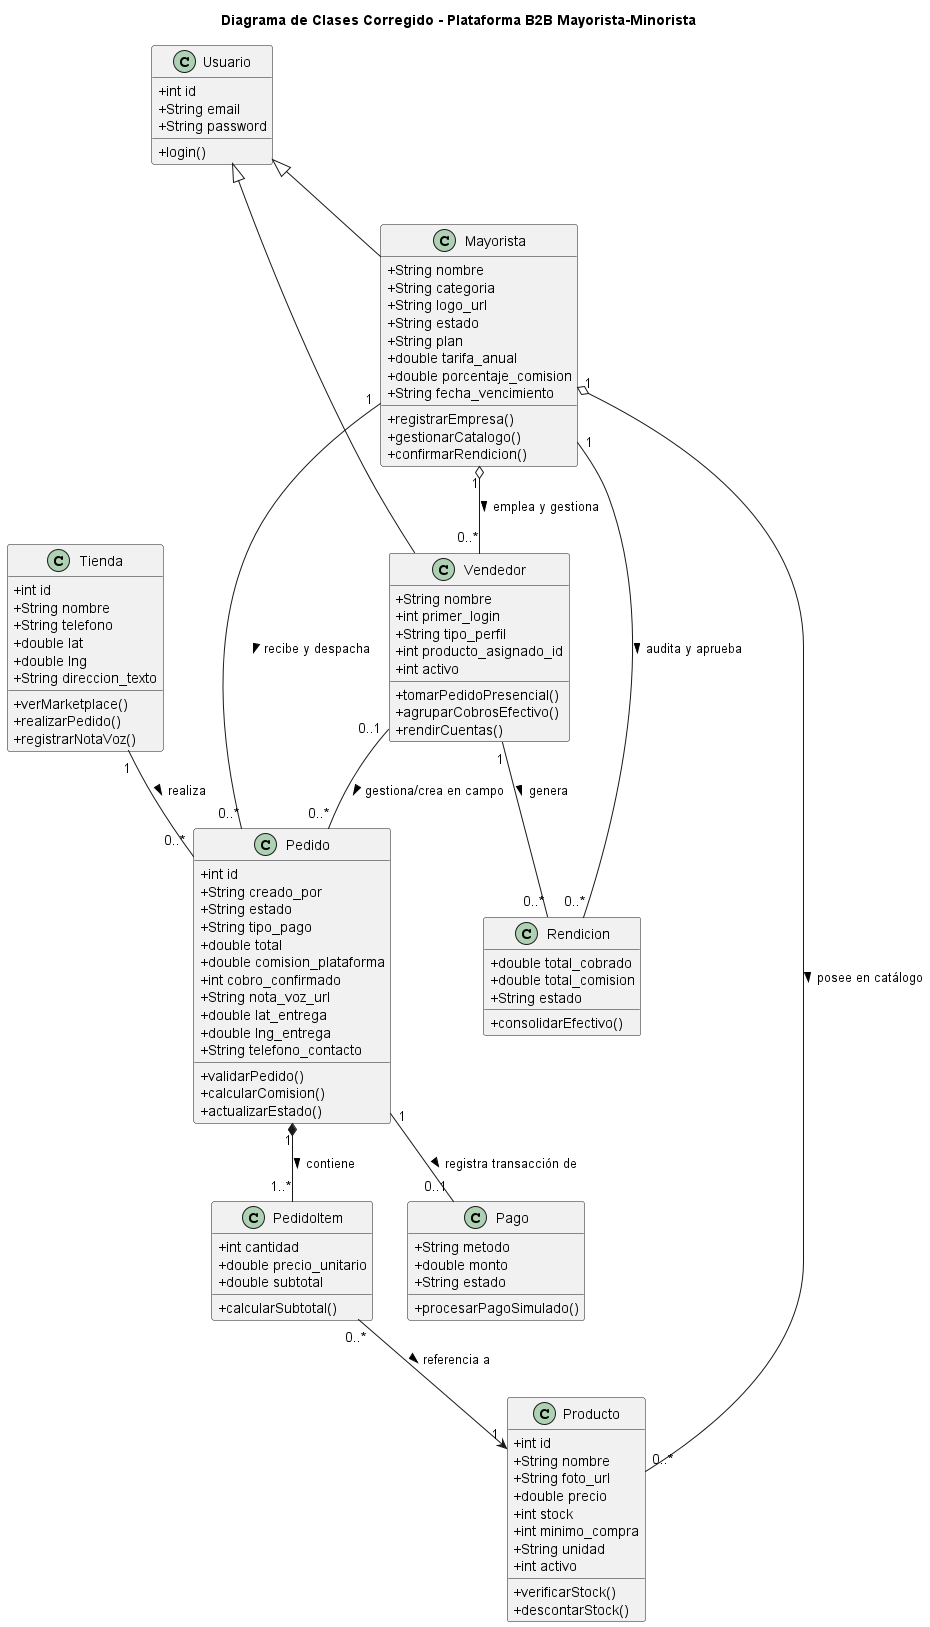
\includegraphics[width=0.75\textwidth]{image1.png}
  \caption{Diagrama de Clases}
\end{figure}

\textbf{Diagrama de BD:}

\begin{figure}[H]
  \centering
  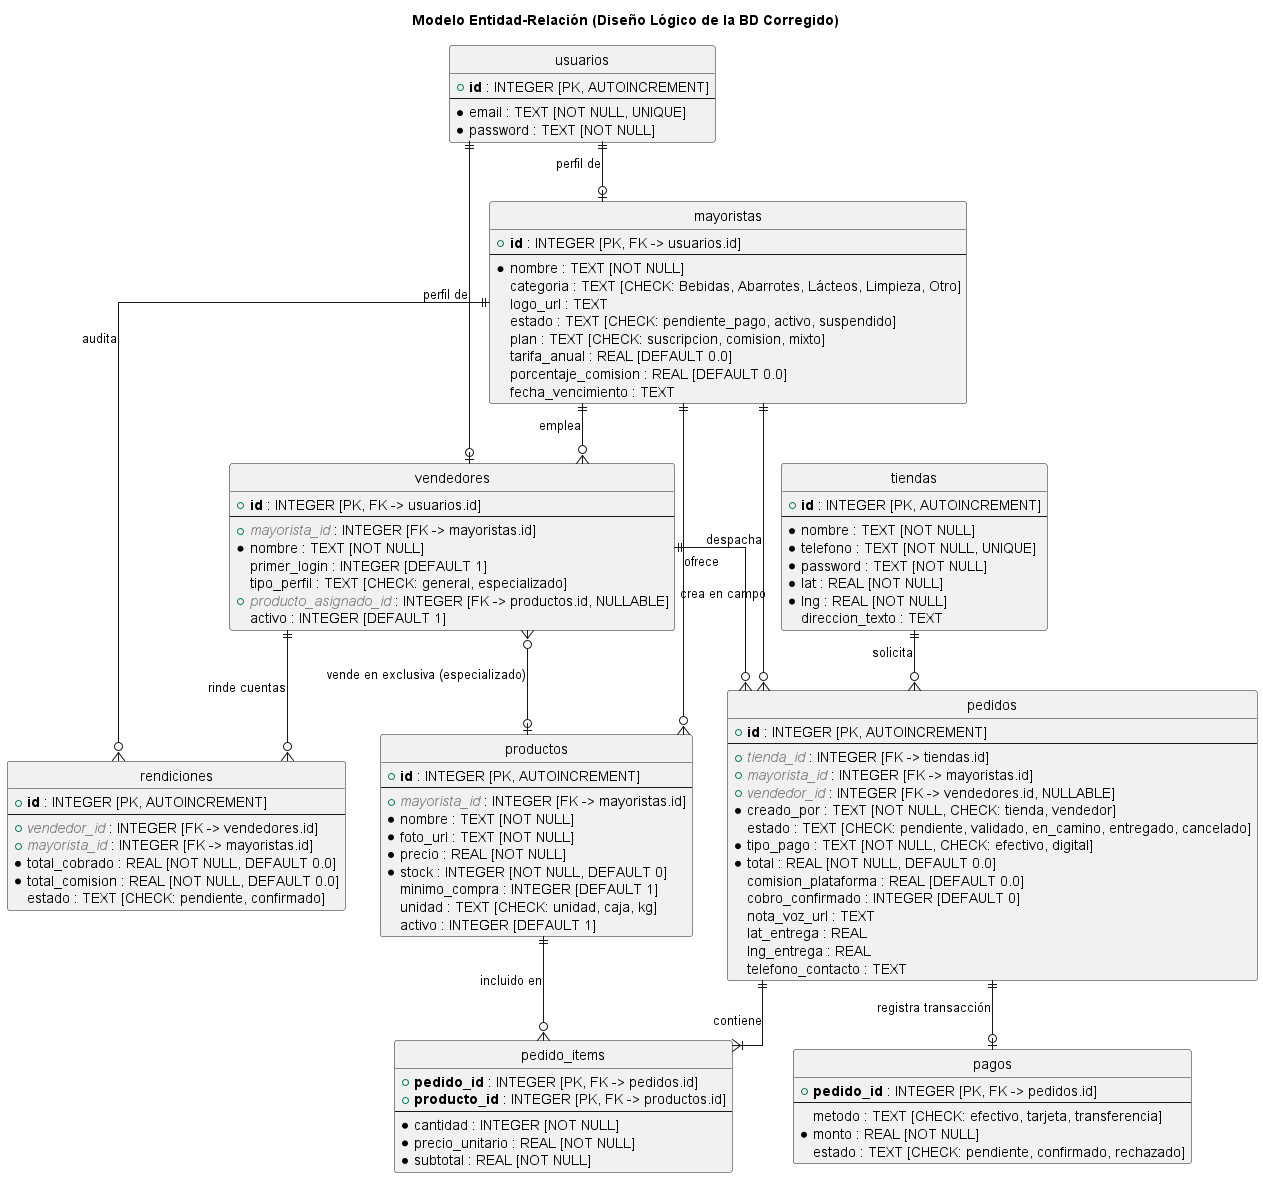
\includegraphics[width=0.85\textwidth]{image2.png}
  \caption{Diagrama de Base de Datos}
\end{figure}

\textbf{1. ¿Cómo se manejan los diferentes tipos de usuarios sin duplicar datos?}

Mediante herencia por tabla. Existe una tabla padre \texttt{usuarios} (guarda email y contraseña) y las tablas hijas \texttt{vendedores} y \texttt{mayoristas} comparten el mismo id como Clave Primaria y Foránea a la vez. Esto crea una relación estricta 1 a 1.

\textbf{2. ¿Cómo se evita que dos clientes compren un producto al mismo tiempo y lo dejen sin stock?}

En el backend de Django, la creación del pedido está envuelta en el decorador \texttt{@transaction.atomic()}. Esto bloquea temporalmente las filas en la base de datos SQLite durante la compra. Si el stock no alcanza, se cancela todo el proceso (Rollback) y se arroja un error controlado.

\textbf{3. ¿Qué pasa con los ítems de un pedido si este se elimina del sistema?}

Se borran automáticamente en cascada. La tabla \texttt{pedido\_items} utiliza una Clave Primaria Compuesta (\texttt{pedido\_id + producto\_id}) y tiene configurada la restricción \texttt{ON DELETE CASCADE} vinculada al pedido. No quedan datos huérfanos.

\textbf{4. ¿Cómo guarda el sistema la ubicación y los datos del tendero analfabeto sin que escriba texto?}

La tabla \texttt{pedidos} guarda la localización mediante campos flotantes (\texttt{lat\_entrega}, \texttt{lng\_entrega}) capturados desde el mapa interactivo, y la dirección mediante una URL (\texttt{nota\_voz\_url}) que apunta a un archivo de audio grabado por el usuario.

\textbf{5. ¿Por qué usar SQLite local en lugar de una base de datos en un servidor independiente?}

Por coste y velocidad. Al ser un único archivo físico (\texttt{db.sqlite3}) alojado en el mismo disco del servidor que el backend de Django, se elimina la latencia de red en las consultas, garantizando tiempos de respuesta menores a 2 segundos sin pagar infraestructura extra.

\subsection{Diagrama de componentes}

\begin{figure}[H]
  \centering
  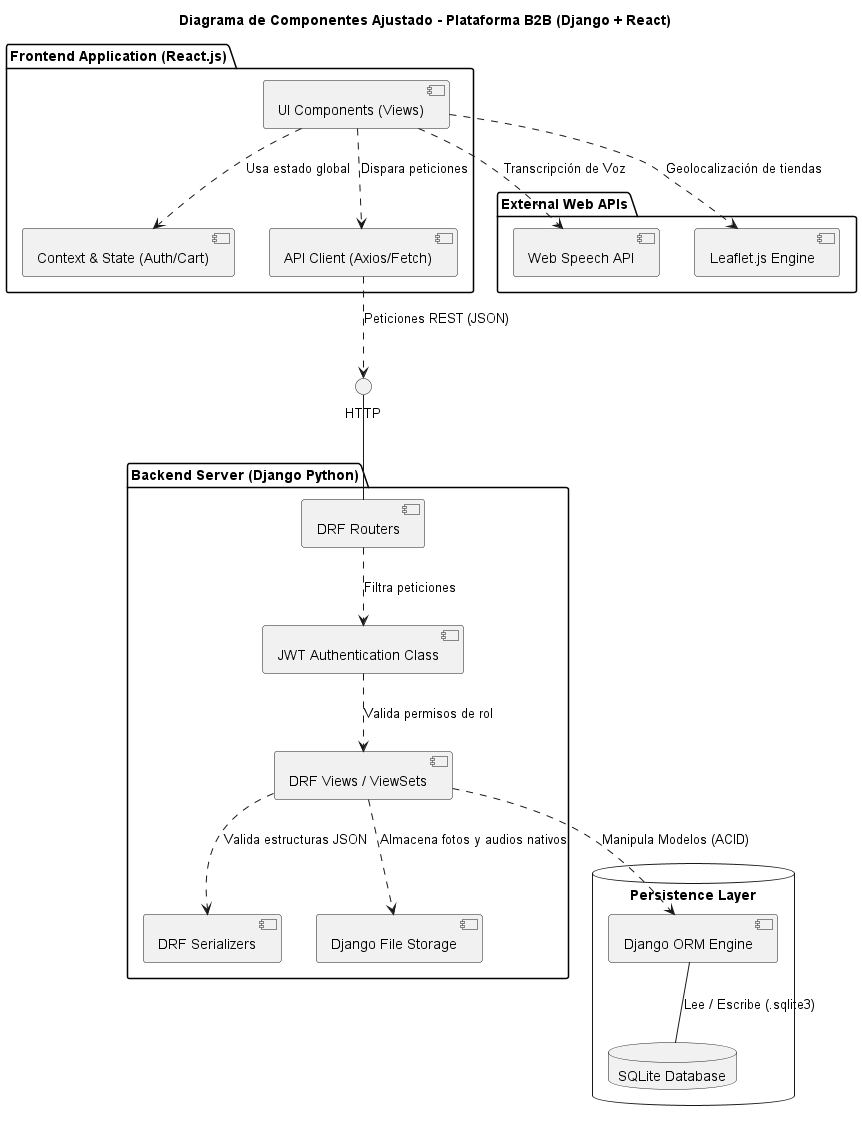
\includegraphics[width=0.85\textwidth]{image3.png}
  \caption{Diagrama de Componentes}
\end{figure}

\subsection{Arquitectura lógica y física (propuesta)}

\subsubsection{Arquitectura Lógica (Multicapa - Decoupled REST Architecture)}

La solución de software se diseña bajo un patrón de \textbf{Arquitectura Multicapa Desacoplada}, segmentando las responsabilidades del sistema en componentes independientes y de alta cohesión. La comunicación entre las fronteras del cliente (Frontend) y el servidor (Backend) se gestiona de forma asíncrona mediante el protocolo HTTP, utilizando JavaScript Object Notation (JSON) como formato estándar de intercambio de datos.

Este enfoque garantiza la mantenibilidad global del sistema (RNF-08) y permite aislar los fallos de un componente sin comprometer la disponibilidad de las demás capas:

\begin{itemize}
  \item \textbf{Capa de Presentación (Frontend - SPA React):} Consiste en una Aplicación de Página Única (Single Page Application) construida en \textbf{React.js} y optimizada visualmente con \textbf{Tailwind CSS} bajo una filosofía \textit{Mobile-First}. Esta capa es la encargada de procesar las interacciones directas de los usuarios (vendedores y tenderos) y renderizar dinámicamente las interfaces gráficas inclusivas basadas en iconos de alta escala (RF-04). Consume las APIs nativas del navegador del dispositivo móvil (\texttt{MediaRecorder} y \texttt{SpeechRecognition}) para empaquetar los flujos de audio y enviarlos en formato binario estructurado multipart de vuelta al servidor.

  \item \textbf{Capa de Exposición de Servicios (Django REST Framework - DRF):} Constituye el punto de entrada controlado hacia el Backend. Se encarga del ruteo inteligente de peticiones mediante el componente DRF Routers y de la interceptación segura de cabeceras HTTP a través de un middleware de autenticación basado en \textbf{JWT} (SimpleJWT), encargándose de decodificar y validar los permisos asociados a cada rol (Mayorista, Vendedor, Tienda) en cada llamada. Utiliza los \textit{Serializers} nativos de DRF para ejecutar la validación sintáctica del JSON entrante y formatear de forma homogénea las respuestas salientes.

  \item \textbf{Capa de Lógica de Negocio (Django Views / ViewSets):} Contiene el núcleo algorítmico y operativo de la plataforma B2B. En esta capa se programan y ejecutan las reglas del negocio complejas, tales como el cálculo dinámico de comisiones del operador en base al tipo de plan contratado, la lógica de consolidación de cobros para las rendiciones físicas de los vendedores y la orquestación transaccional ACID.

  \item \textbf{Capa de Persistencia y Almacenamiento de Datos (Django ORM):} Abstrae la manipulación directa de la base de datos a través de modelos orientados a objetos fuertemente tipados. El \textbf{Django ORM} asegura el aislamiento transaccional inmediato en el motor relacional integrado \textbf{SQLite} ante solicitudes de compra concurrentes. Asimismo, administra automáticamente el almacenamiento físico de recursos estáticos e imágenes a través del subsistema nativo de almacenamiento multimedia de Django (\texttt{FileSystemStorage}) en directorios locales controlados.
\end{itemize}

\subsubsection{Arquitectura Física (Propuesta de Despliegue en Producción)}

Considerando el objetivo de optimización de costos e infraestructura para la escala inicial del proyecto (OBJ-03) y la meta de mantener tiempos de respuesta óptimos (RNF-04), se propone un esquema de despliegue físico modular centralizado basado en un Servidor Virtual Privado (VPS) robusto:

\begin{itemize}
  \item \textbf{Servidor de Aplicación Virtualizado (VPS):} Se despliega una instancia cloud corriendo bajo una distribución de Linux orientada a servidores (\textbf{Ubuntu Server}). Los requerimientos de hardware mínimos calculados para tolerar la concurrencia de la red de minoristas son:
  \begin{itemize}
    \item \textbf{CPU:} 1 o 2 vCPUs de cómputo dedicado.
    \item \textbf{Memoria RAM:} 2 GB.
    \item \textbf{Almacenamiento:} 20 GB SSD de alta velocidad (necesarios para alojar el archivo dinámico relacional y la carpeta persistente \texttt{/media/} administrada por Django para las fotos de catálogo y audios).
  \end{itemize}

  \item \textbf{Servidor Web Frontal y Proxy Inverso (Nginx):} Se sitúa en la frontera física de la red interceptando el tráfico externo por los puertos públicos 80 (HTTP) y 443 (HTTPS) bajo protección de certificados de cifrado \textbf{SSL/TLS Let's Encrypt} (RNF-02). Nginx cumple una doble función física:
  \begin{itemize}
    \item Servir de manera directa y con mínima latencia los archivos estáticos estables compilados del Frontend (HTML, JS, CSS de React) y los recursos multimedia locales de Django sin recargar el hilo del servidor de ejecución.
    \item Actuar como proxy inverso interceptando todas las peticiones que apunten al patrón de ruta \texttt{/api/*} para derivarlas internamente.
  \end{itemize}

  \item \textbf{Servidor de Aplicaciones WSGI (Gunicorn):} Dado que Django es un entorno síncrono por defecto basado en Python, no se ejecuta directamente expuesto a la red. Se implementa \textbf{Gunicorn} como un servidor de procesos HTTP WSGI intermedio. Gunicorn gestiona múltiples hilos de ejecución (\textit{Workers}) en el puerto local cerrado 8000, recibiendo las solicitudes redirigidas por Nginx y ejecutando la lógica dinámica en el entorno de Python de manera concurrente y eficiente.

  \item \textbf{Almacenamiento Relacional Embebido (SQLite Engine):} A diferencia de arquitecturas tradicionales que requieren un clúster físico independiente para la base de datos (como PostgreSQL remoto), al utilizar \textbf{SQLite} el motor y los datos residen en un archivo binario indexado de lectura directa en el mismo disco SSD del VPS (\texttt{db.sqlite3}). Al ejecutarse en el mismo espacio de memoria en disco que el backend de Django, se elimina por completo la latencia de red en las consultas SQL, optimizando radicalmente el rendimiento de las lecturas masivas del marketplace (RNF-04).
\end{itemize}

\subsection{Prototipo de pantallas no funcional}

\textbf{Link del prototipo:} \url{https://wholesale-platform--romerojoelya.replit.app}

\textbf{Credenciales de prueba:} \url{https://drive.google.com/file/d/1FI_932e9UU-dHqA4TcE2mHI8A8WDARh0/view?usp=sharing}

\subsubsection*{Pantallas prototipo}

\begin{figure}[H]
  \centering
  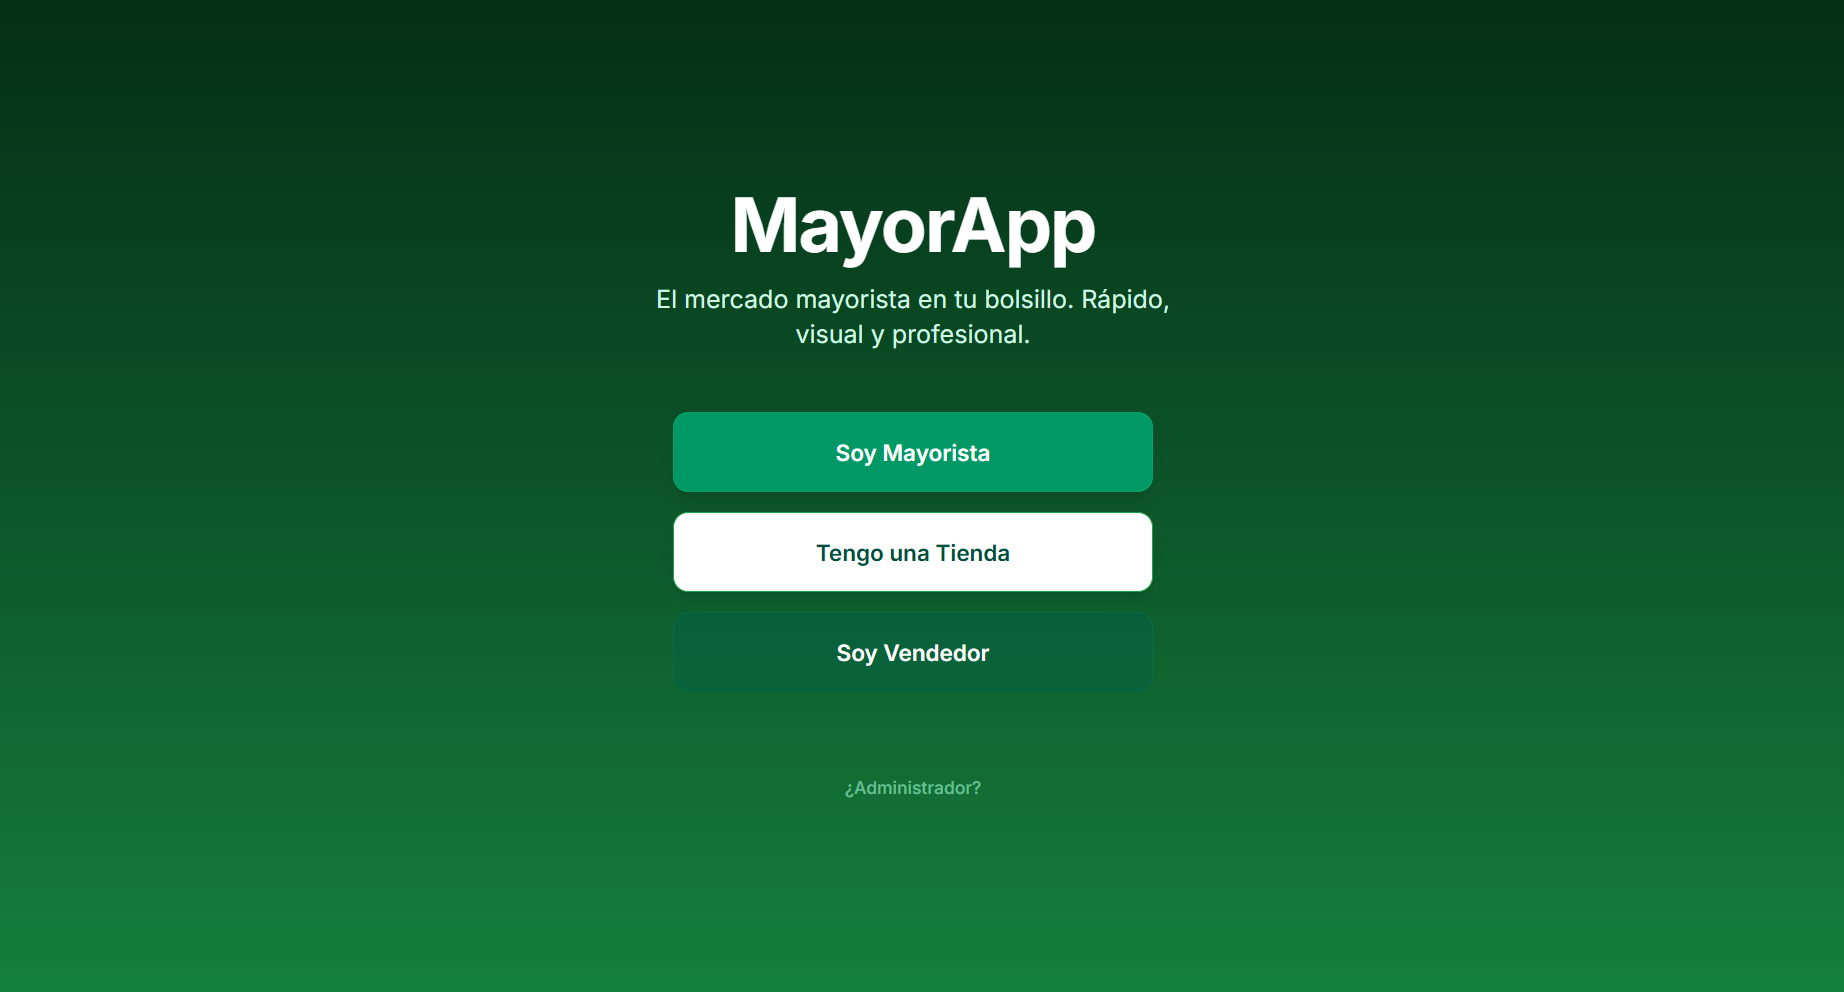
\includegraphics[width=0.9\textwidth]{image4.png}
  \caption*{Vista general -- Inicio de sesión}
\end{figure}

\paragraph{Mayorista:}

\begin{figure}[H]
  \centering
  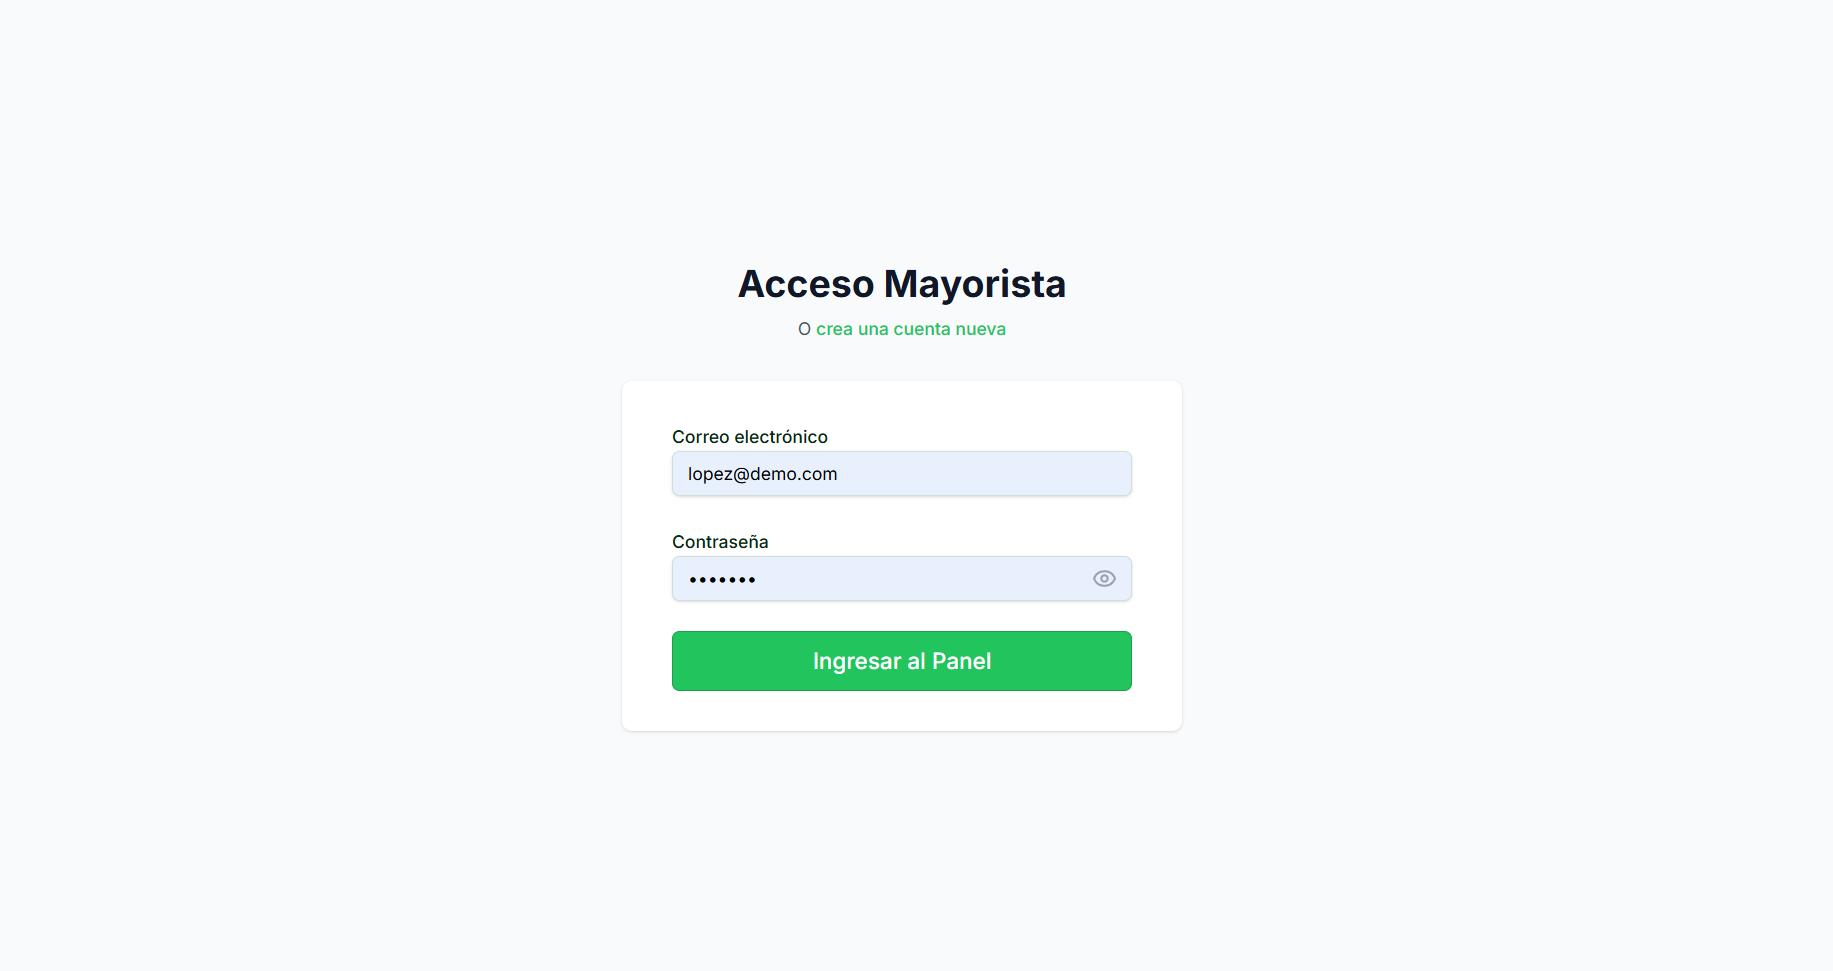
\includegraphics[width=0.9\textwidth]{image5.png}
  \caption*{Mayorista -- Registro de empresa}
\end{figure}
\begin{figure}[H]
  \centering
  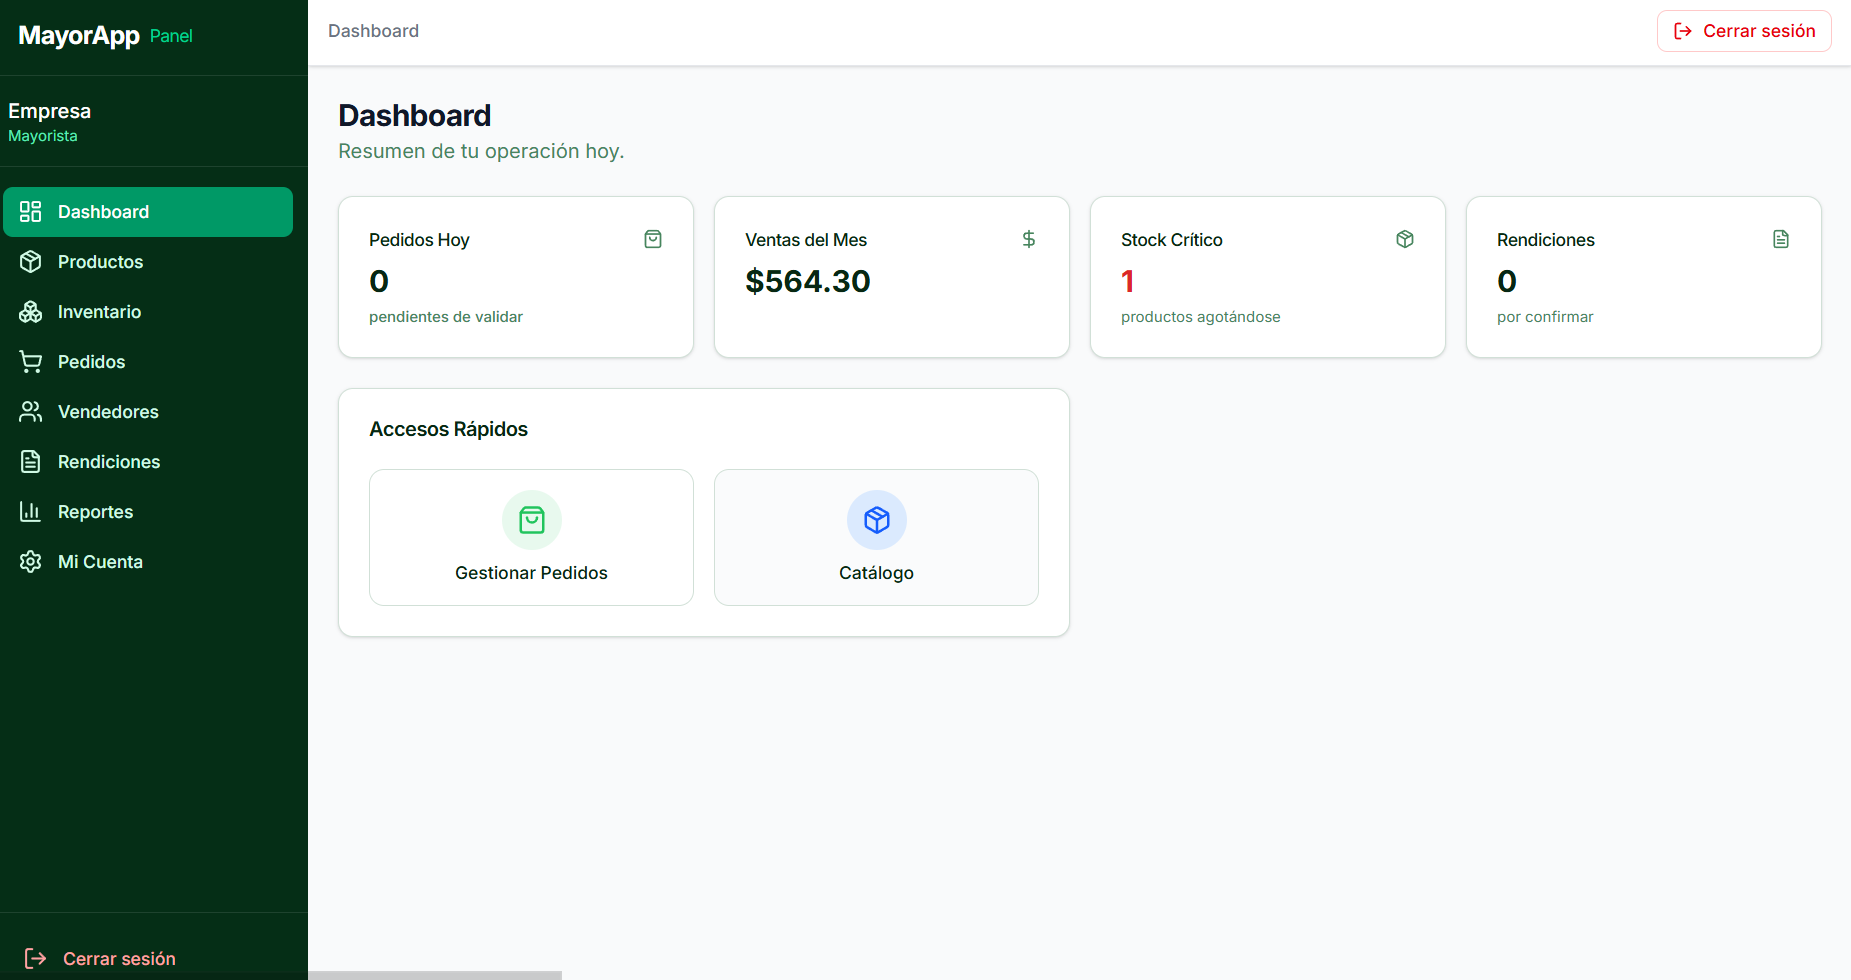
\includegraphics[width=0.9\textwidth]{image6.png}
  \caption*{Mayorista -- Dashboard}
\end{figure}
\begin{figure}[H]
  \centering
  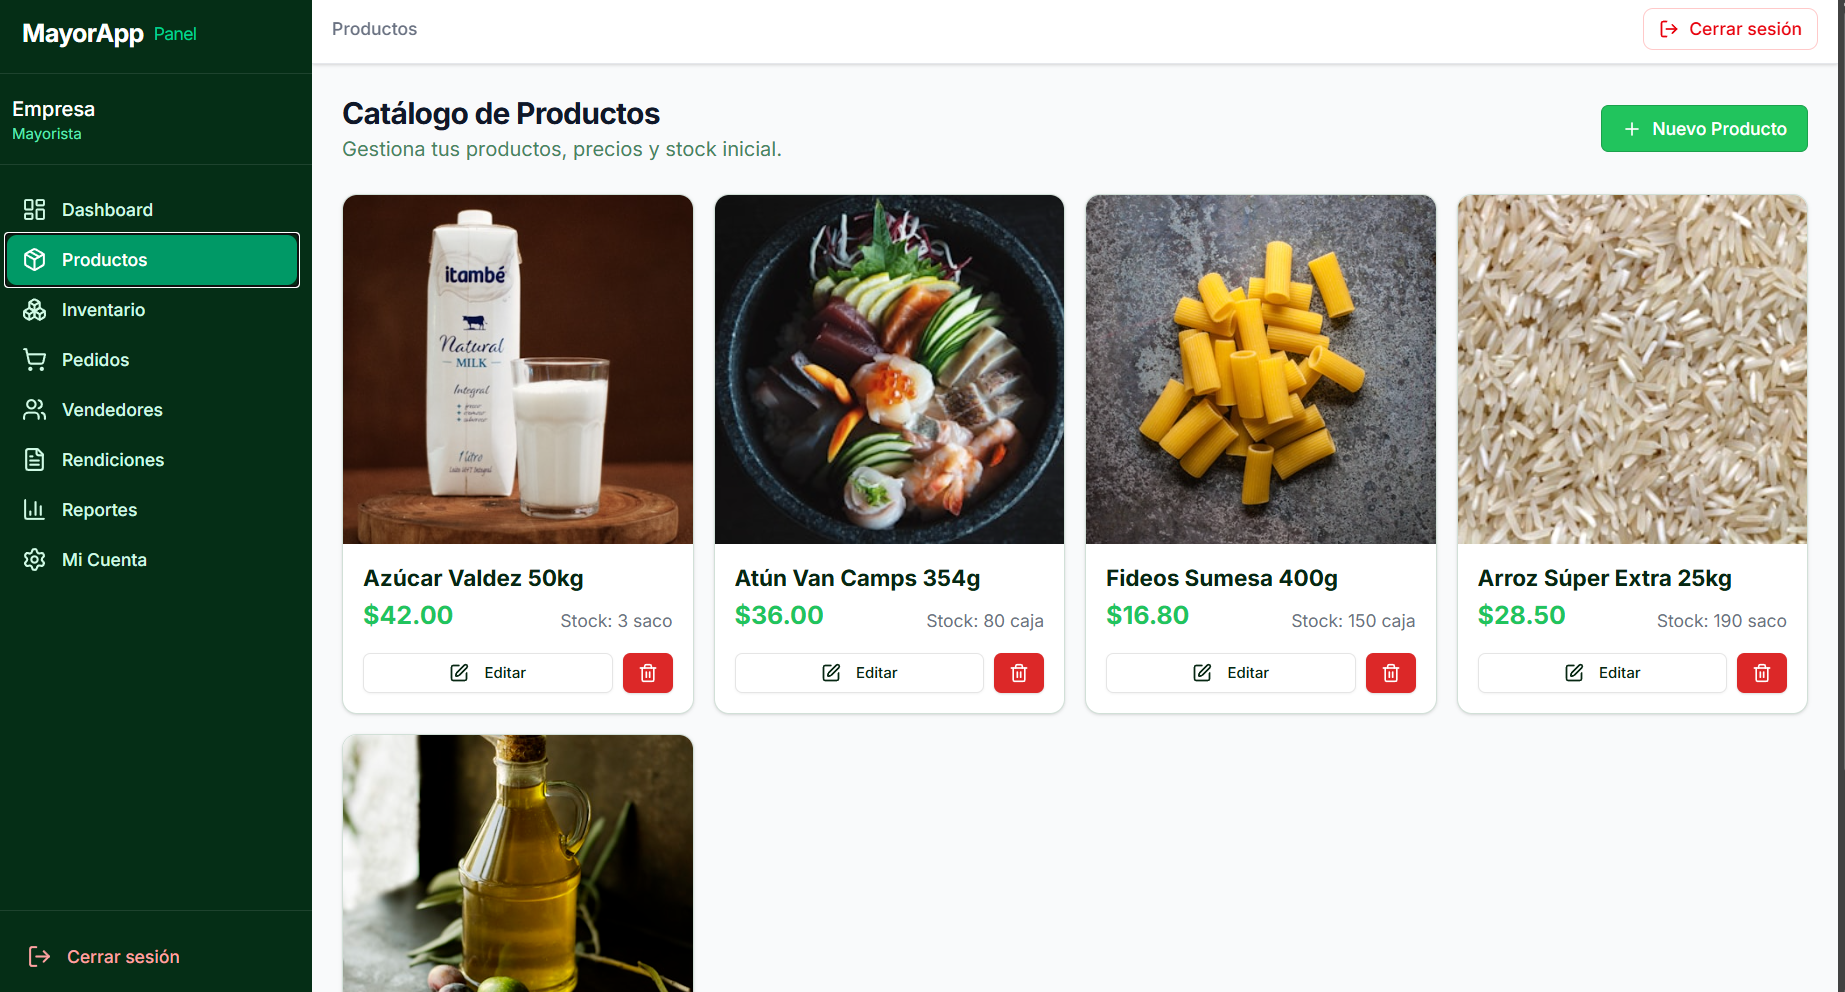
\includegraphics[width=0.9\textwidth]{image7.png}
  \caption*{Mayorista -- Catálogo de Productos}
\end{figure}
\begin{figure}[H]
  \centering
  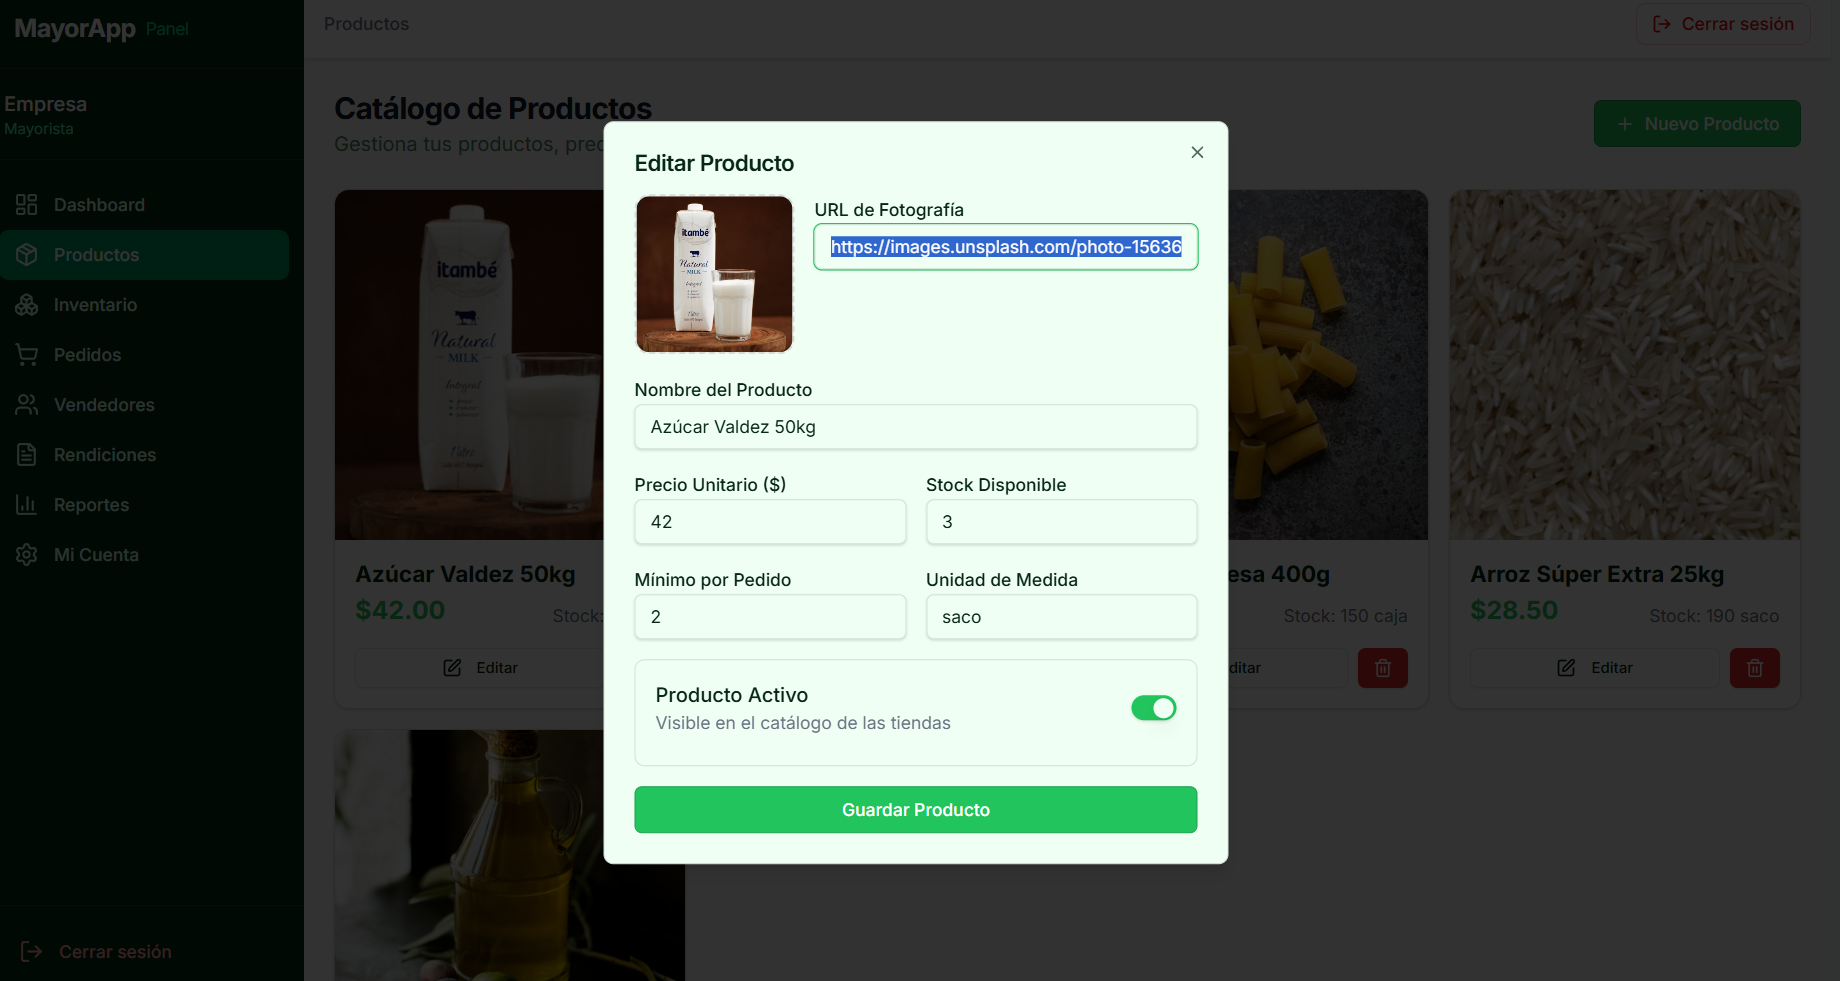
\includegraphics[width=0.9\textwidth]{image8.png}
  \caption*{Mayorista -- Nuevo Producto}
\end{figure}
\begin{figure}[H]
  \centering
  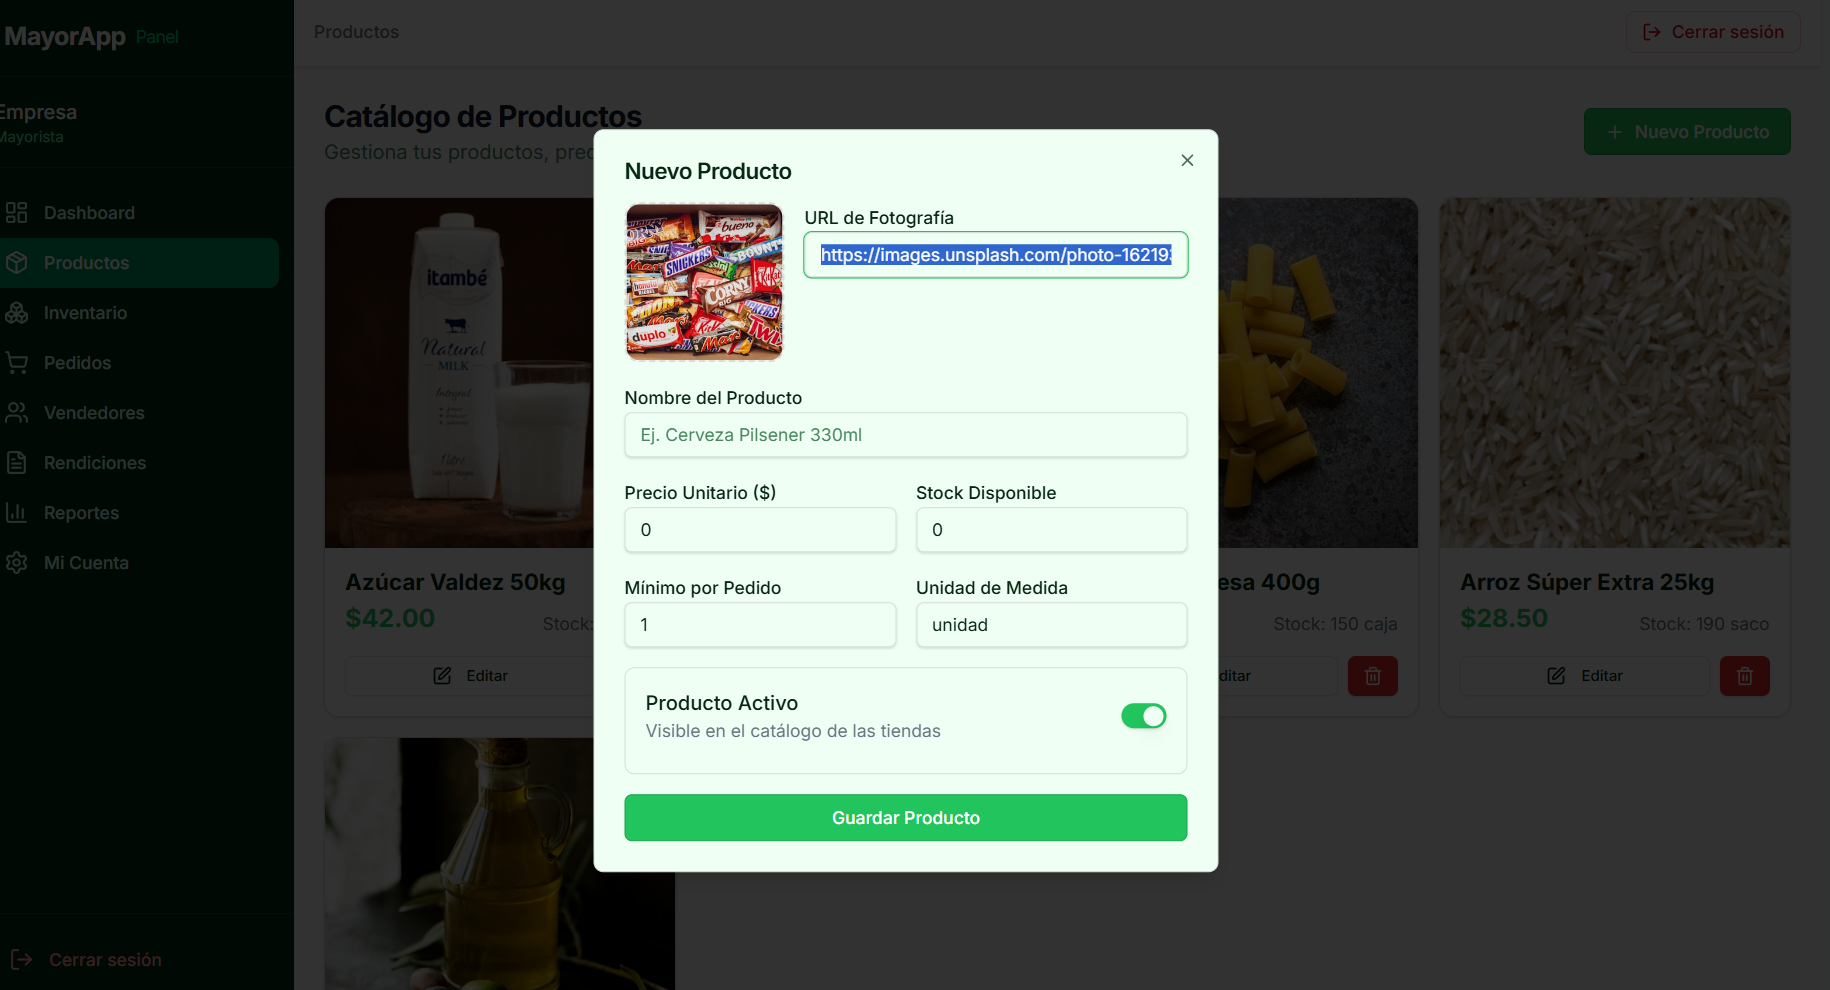
\includegraphics[width=0.9\textwidth]{image9.png}
  \caption*{Mayorista -- Gestión de Pedidos}
\end{figure}
\begin{figure}[H]
  \centering
  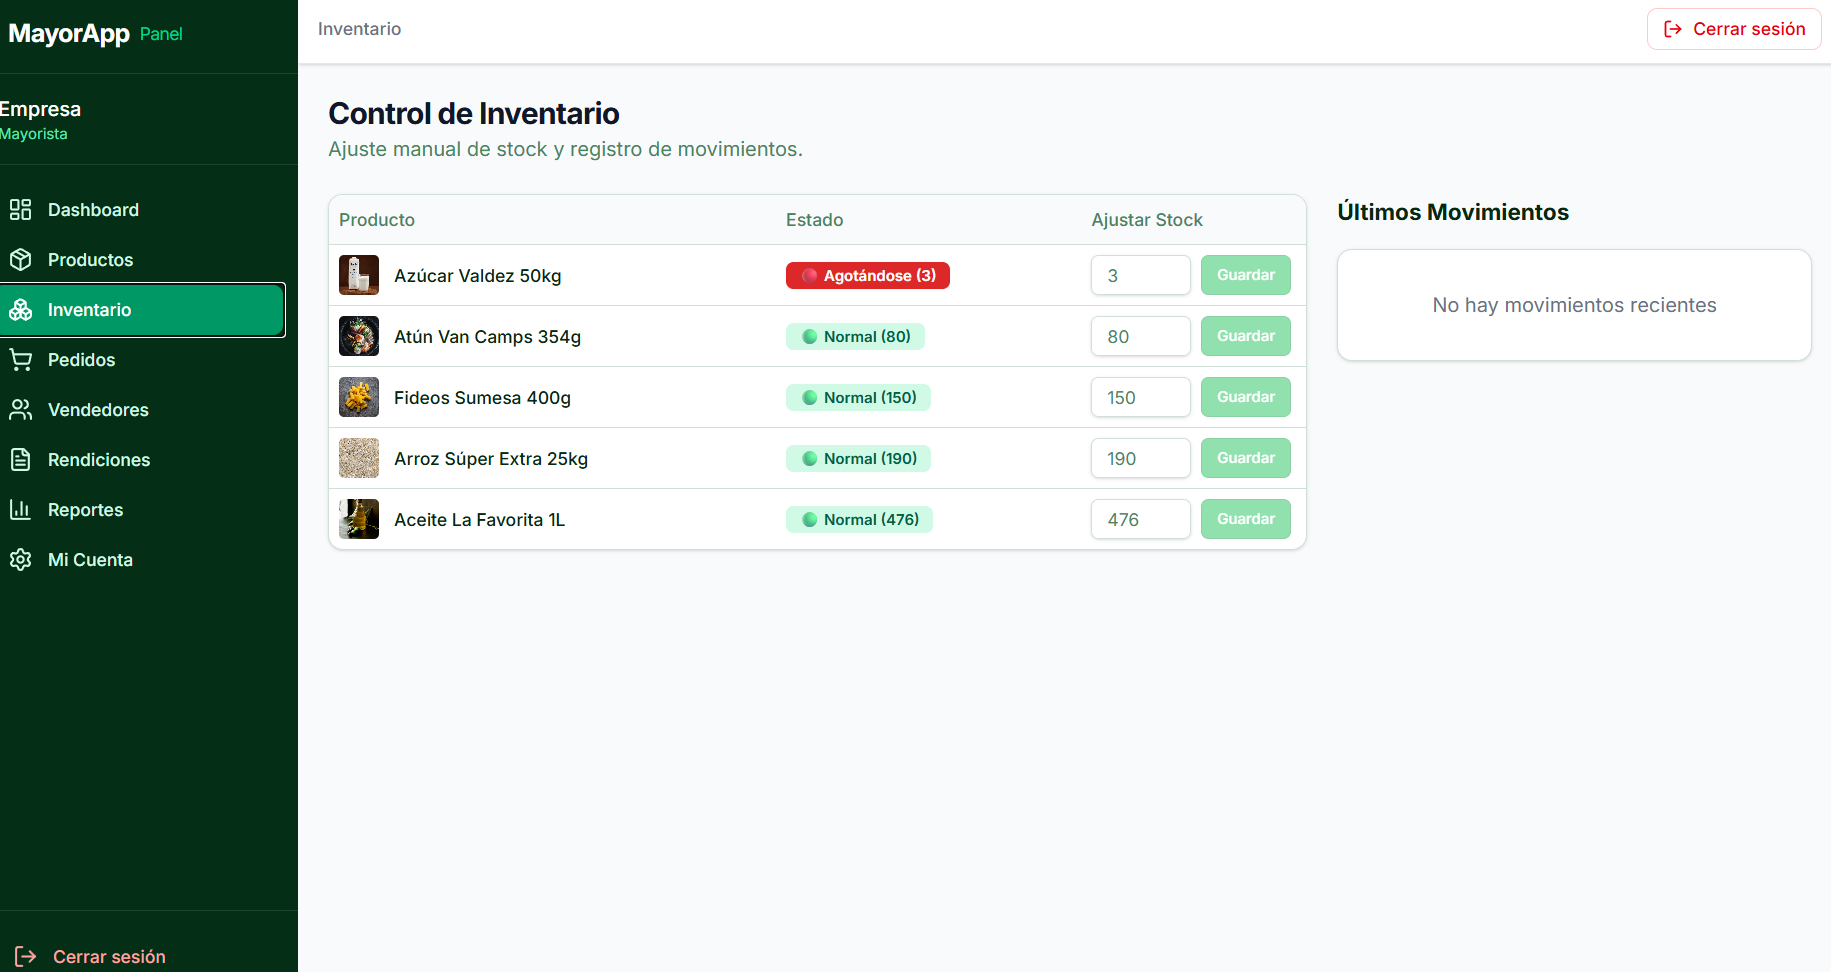
\includegraphics[width=0.9\textwidth]{image10.png}
  \caption*{Mayorista -- Control de Inventario}
\end{figure}
\begin{figure}[H]
  \centering
  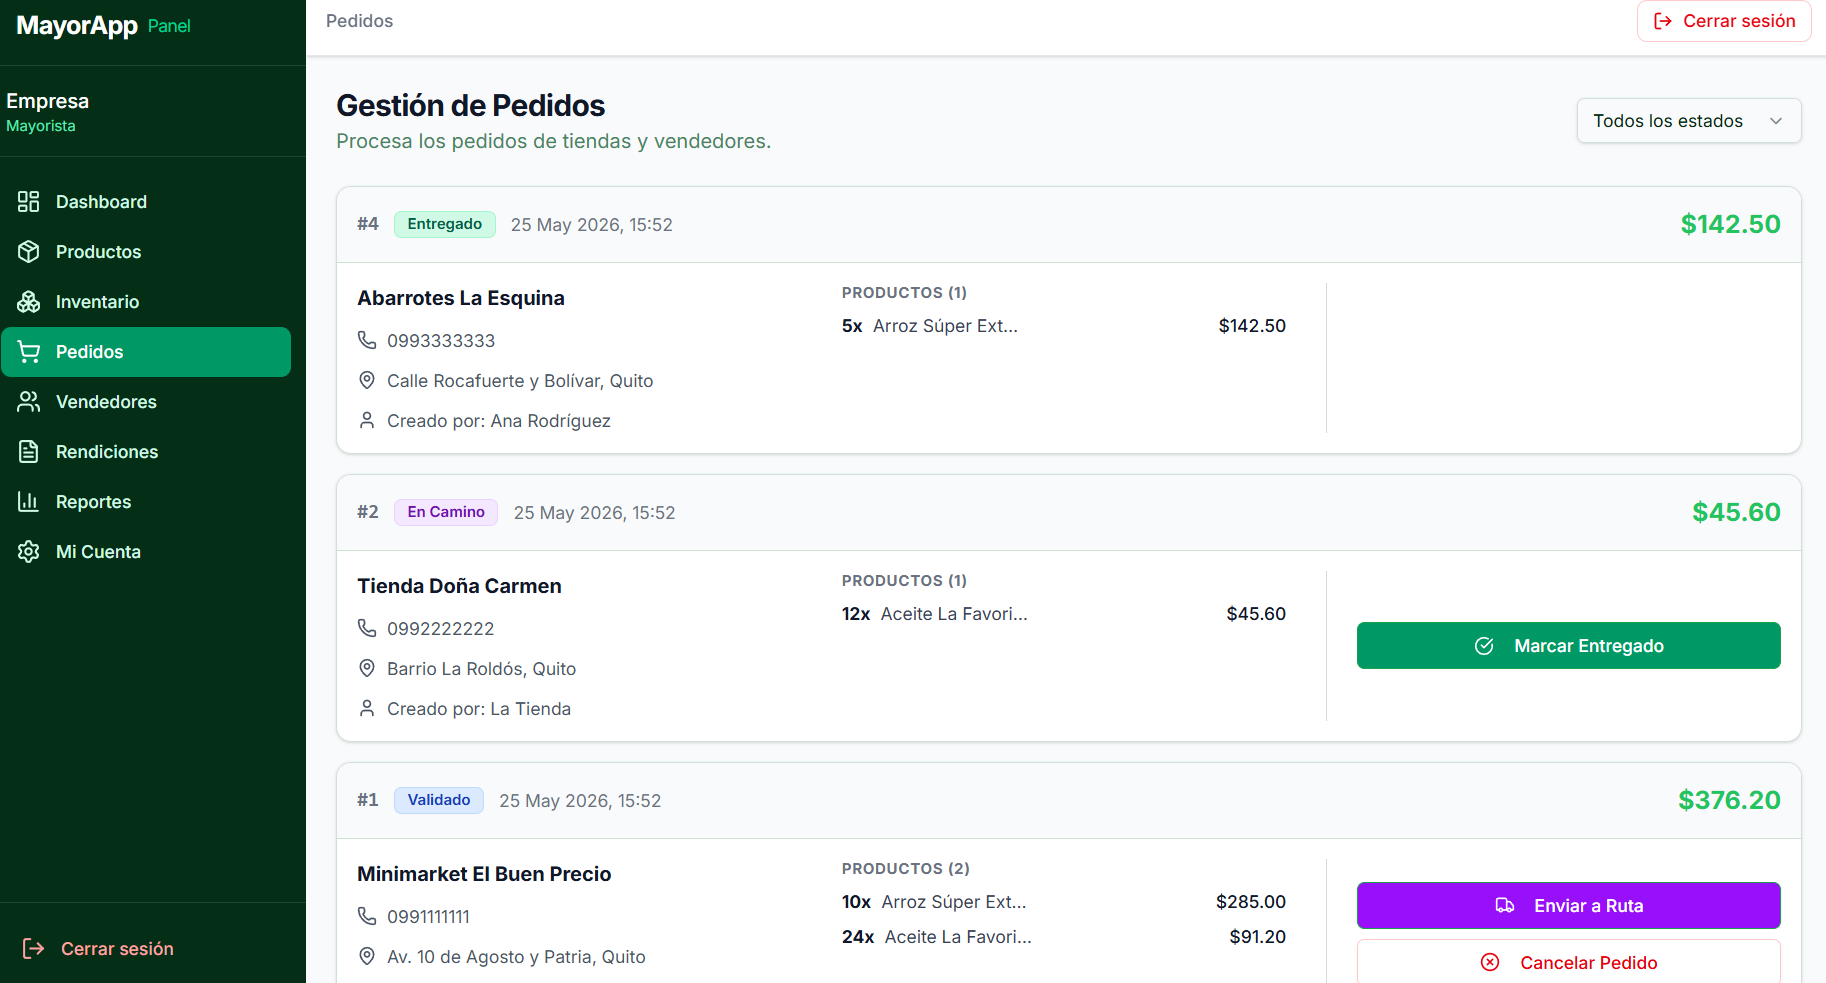
\includegraphics[width=0.9\textwidth]{image11.png}
  \caption*{Mayorista -- Gestión de Pedidos (detalle)}
\end{figure}
\begin{figure}[H]
  \centering
  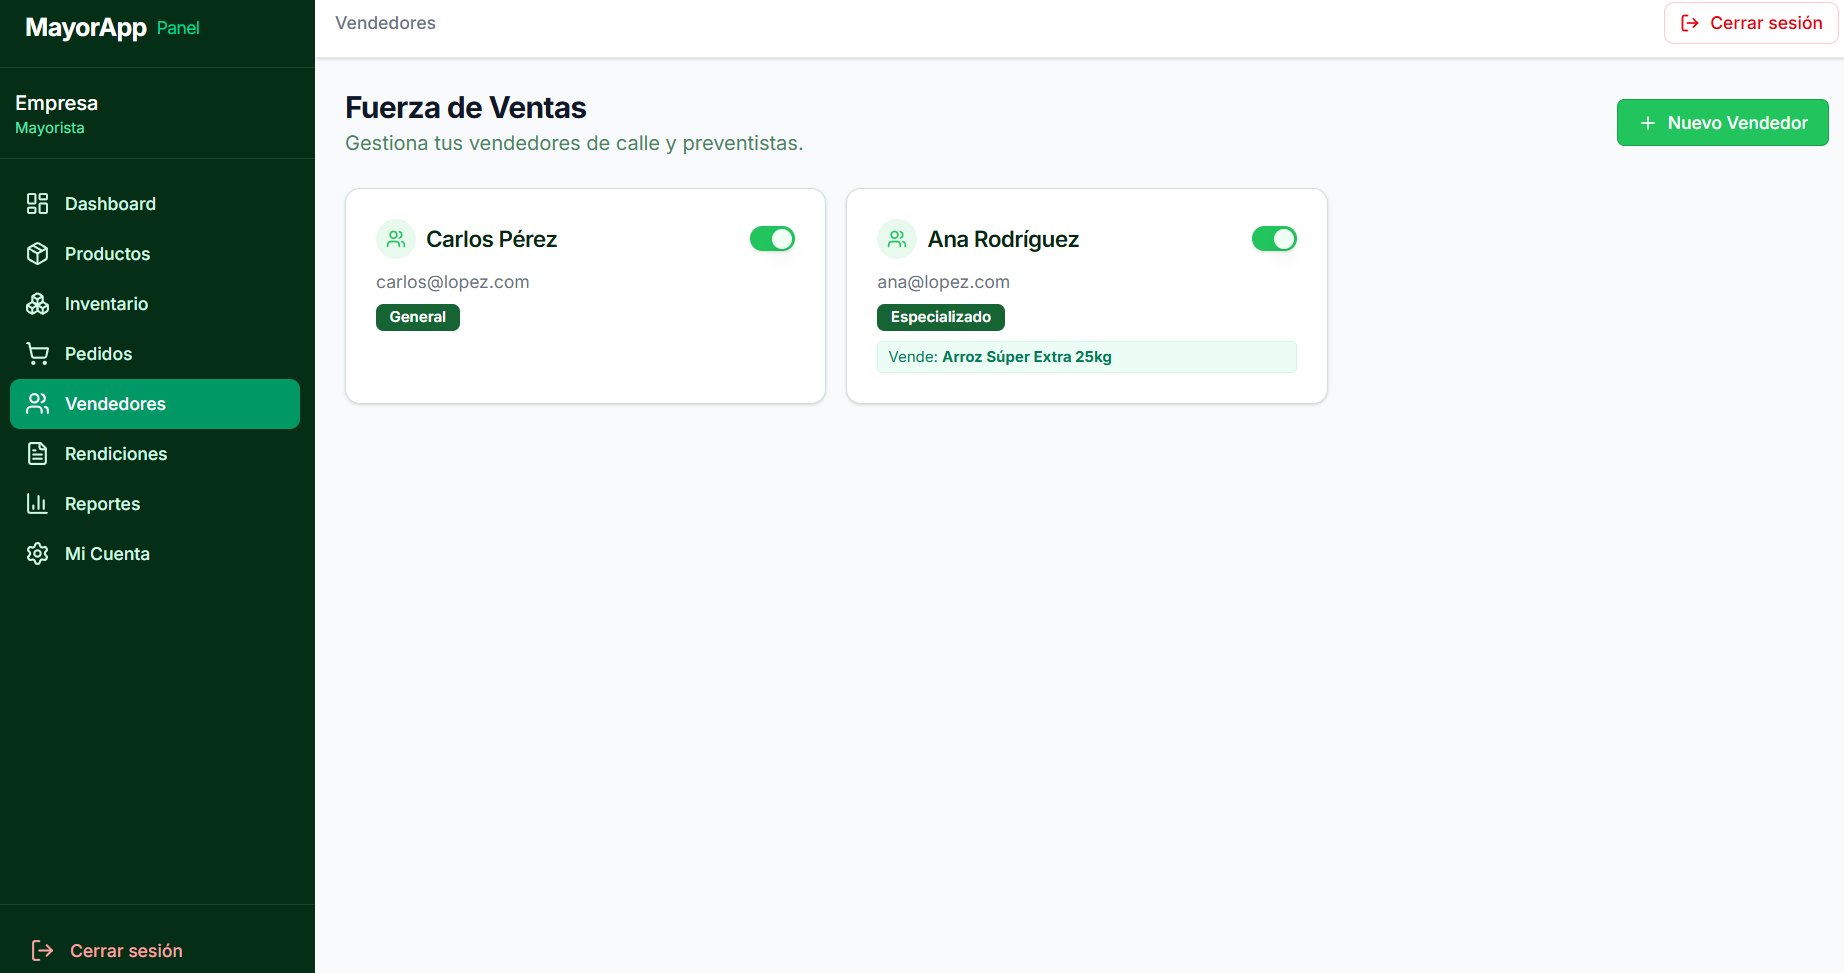
\includegraphics[width=0.9\textwidth]{image12.png}
  \caption*{Mayorista -- Fuerza de Ventas (Vendedores)}
\end{figure}
\begin{figure}[H]
  \centering
  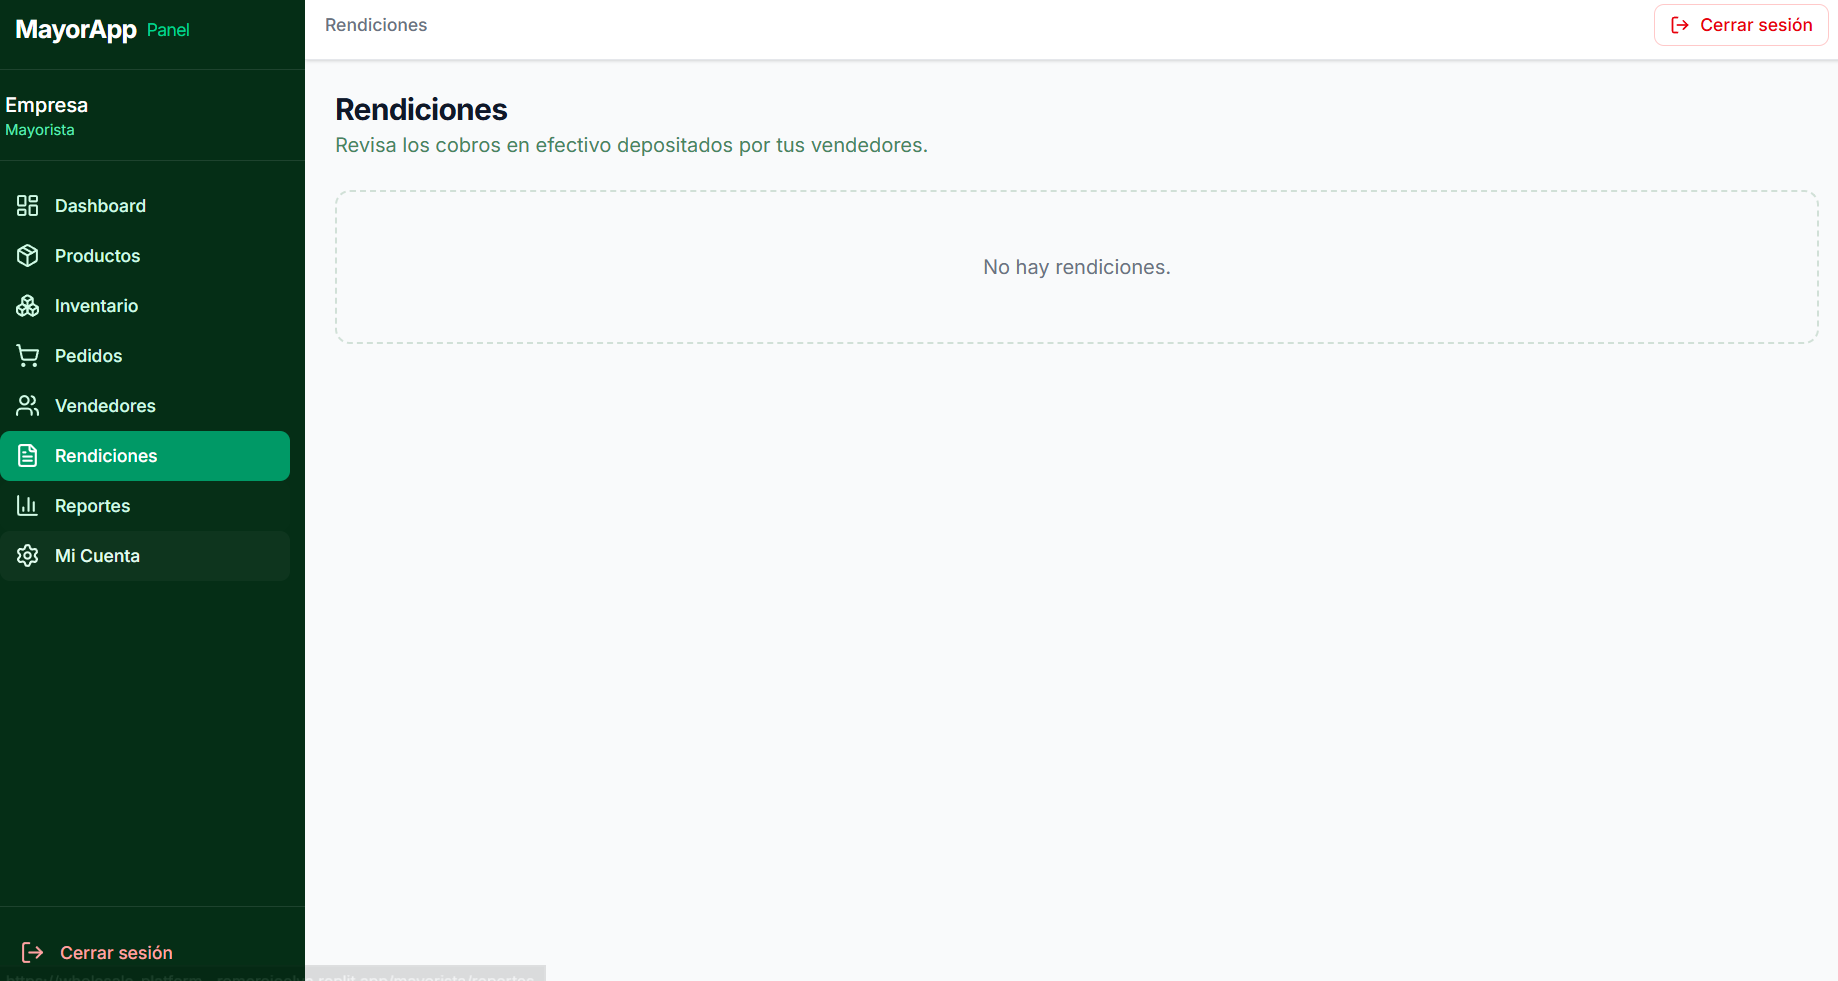
\includegraphics[width=0.9\textwidth]{image13.png}
  \caption*{Mayorista -- Rendiciones}
\end{figure}
\begin{figure}[H]
  \centering
  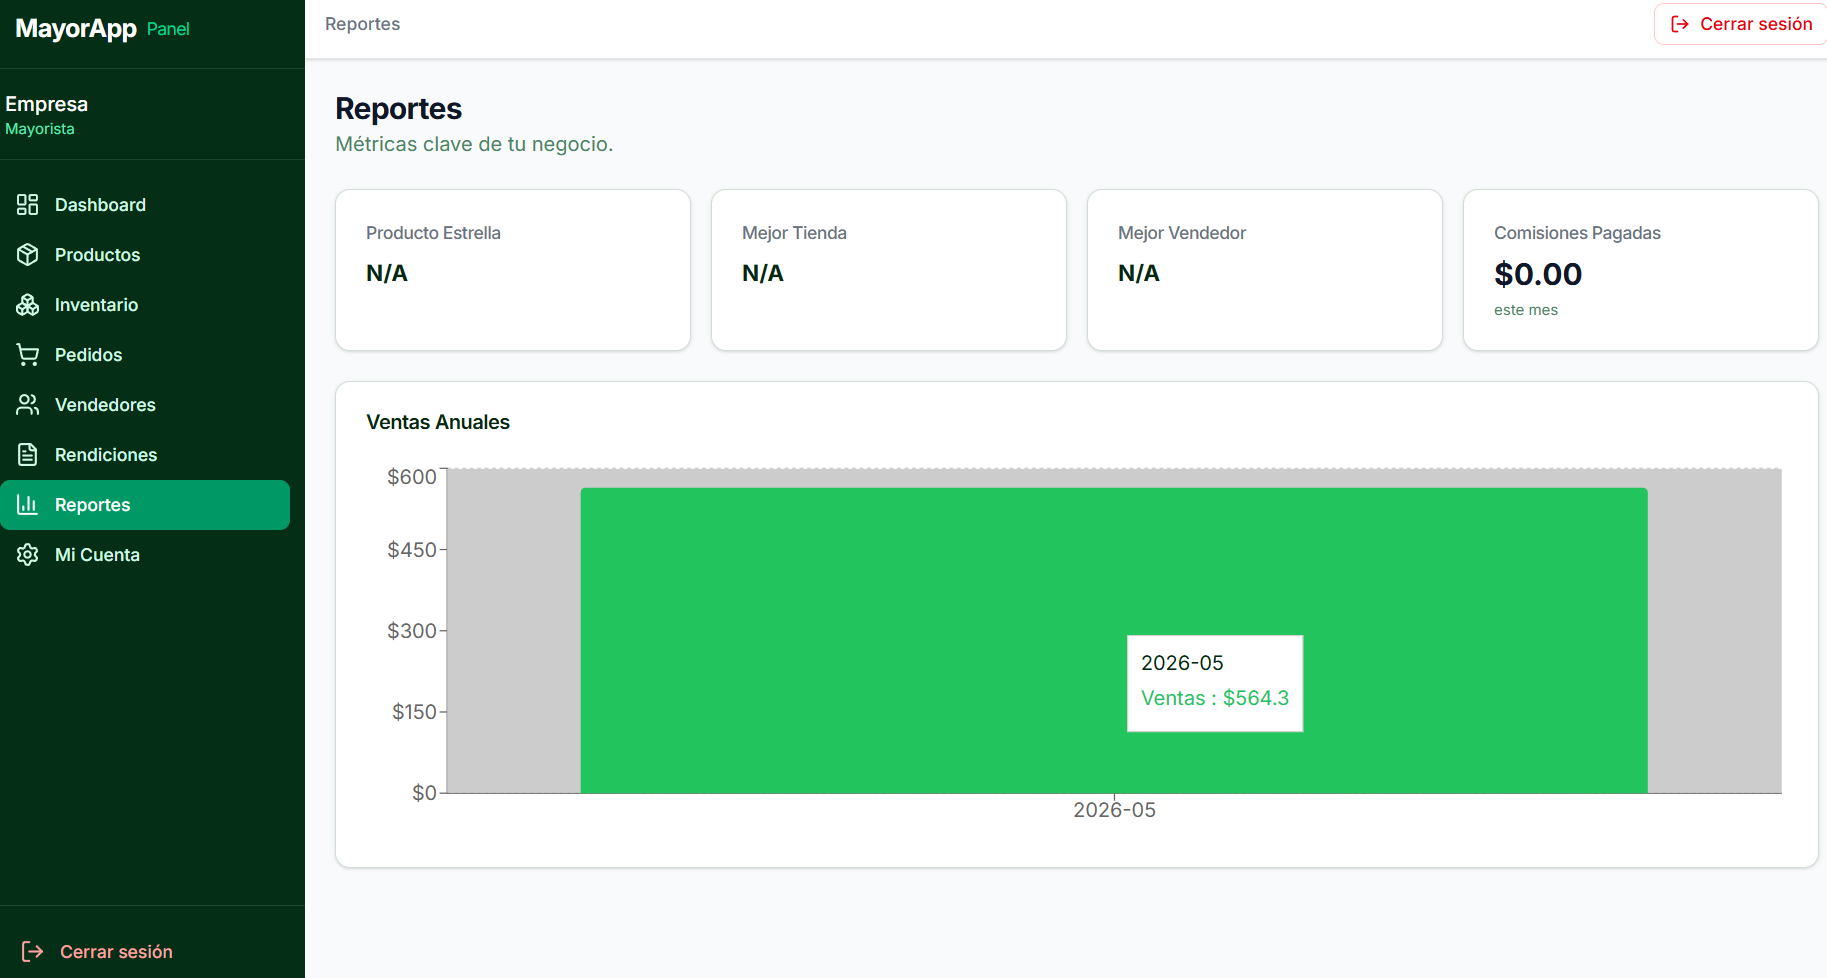
\includegraphics[width=0.9\textwidth]{image14.png}
  \caption*{Mayorista -- Reportes}
\end{figure}
\begin{figure}[H]
  \centering
  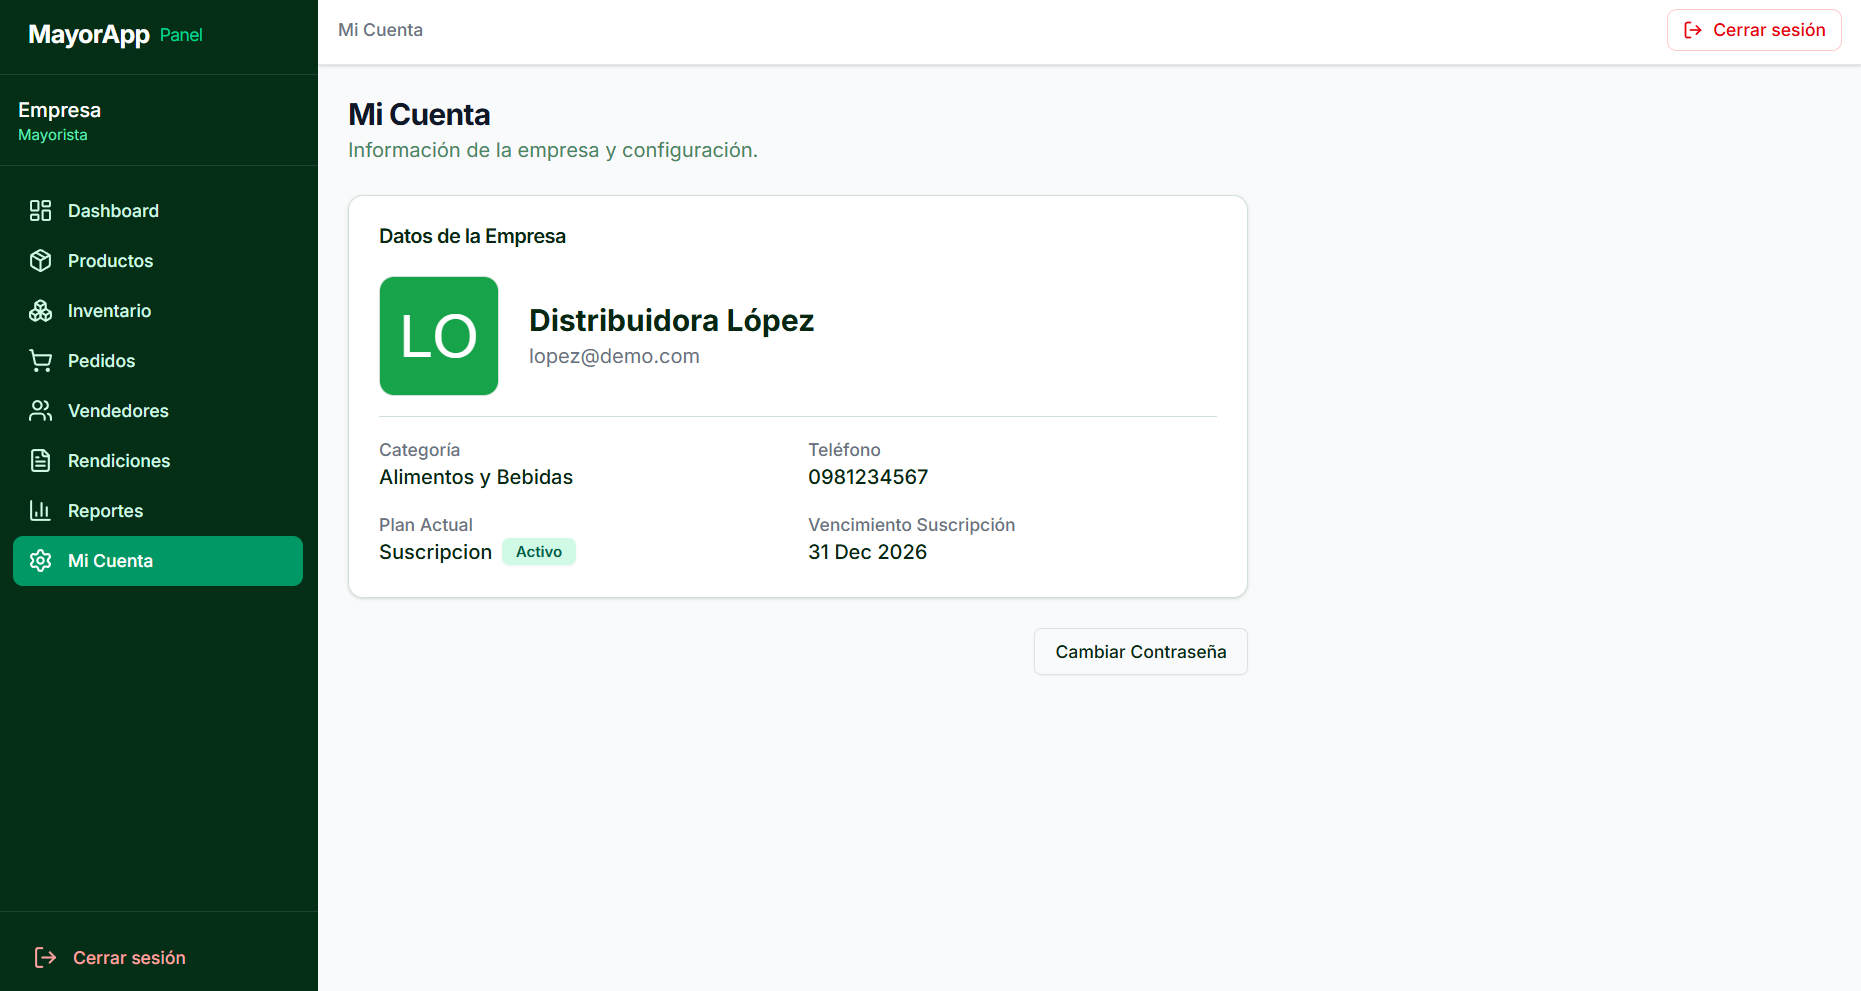
\includegraphics[width=0.9\textwidth]{image15.png}
  \caption*{Mayorista -- Mi Cuenta}
\end{figure}

\paragraph{Tienda:}

\begin{figure}[H]
  \centering
  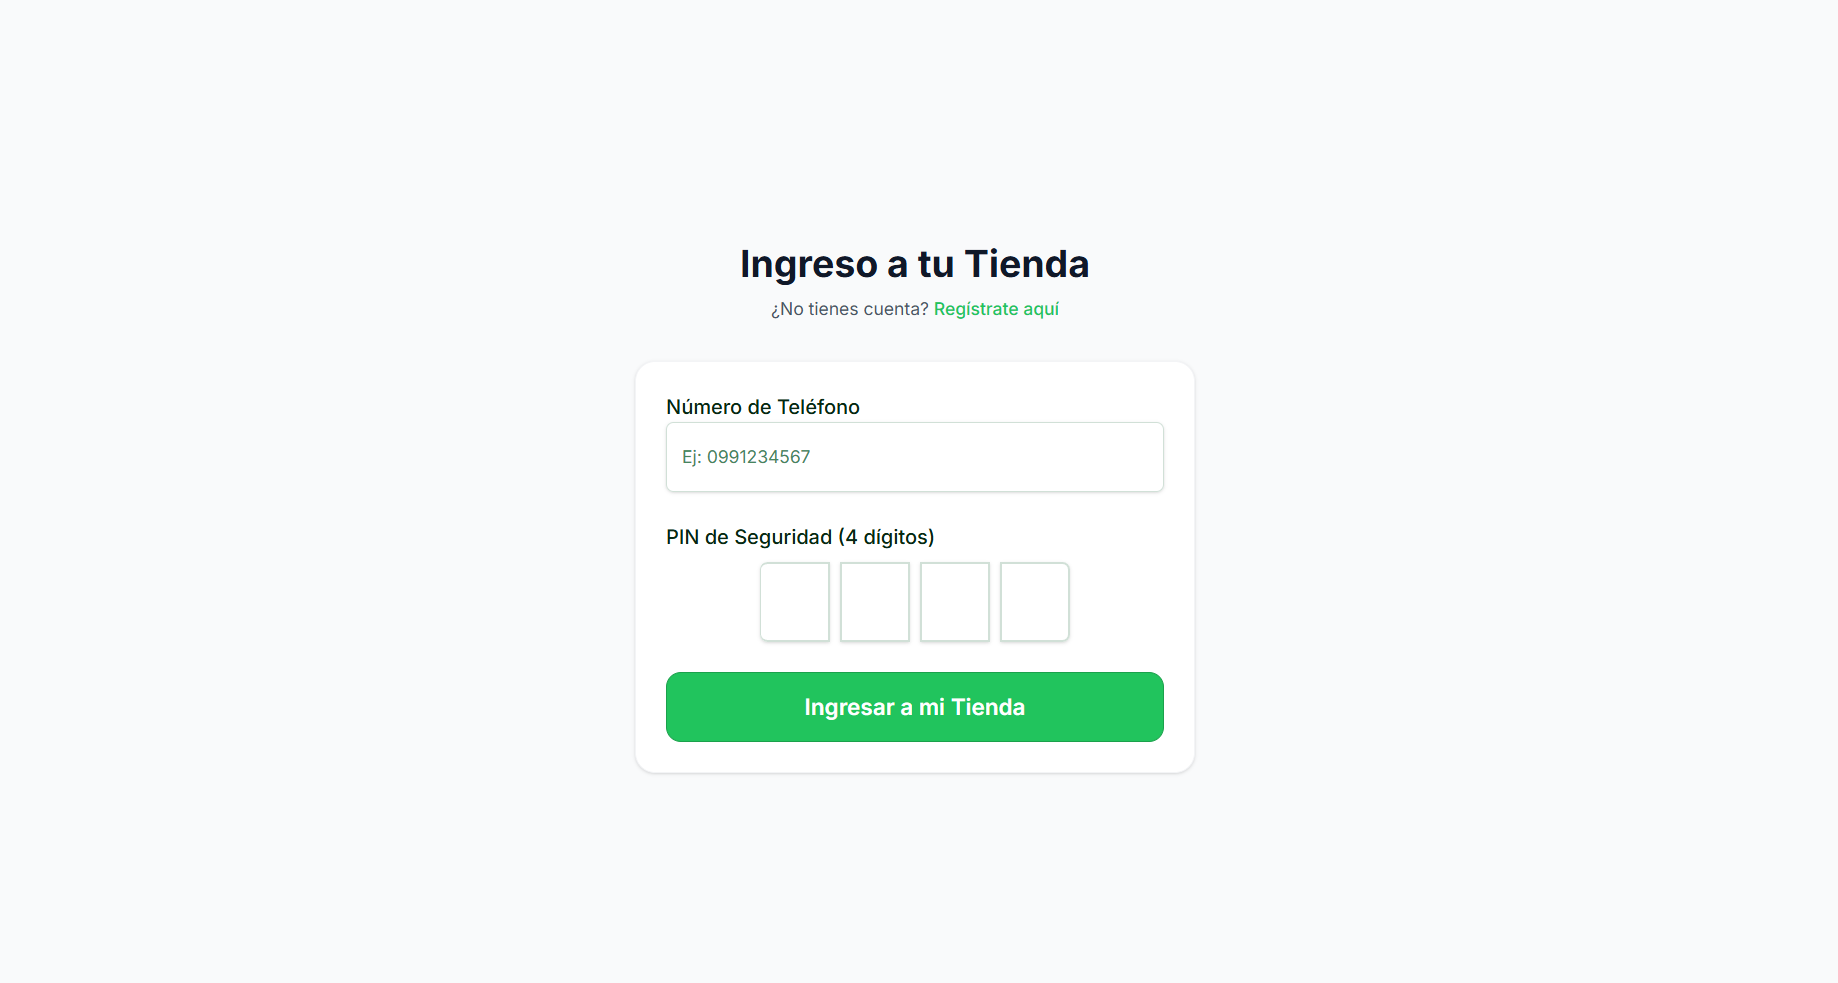
\includegraphics[width=0.9\textwidth]{image16.png}
  \caption*{Tienda -- Inicio de sesión}
\end{figure}
\begin{figure}[H]
  \centering
  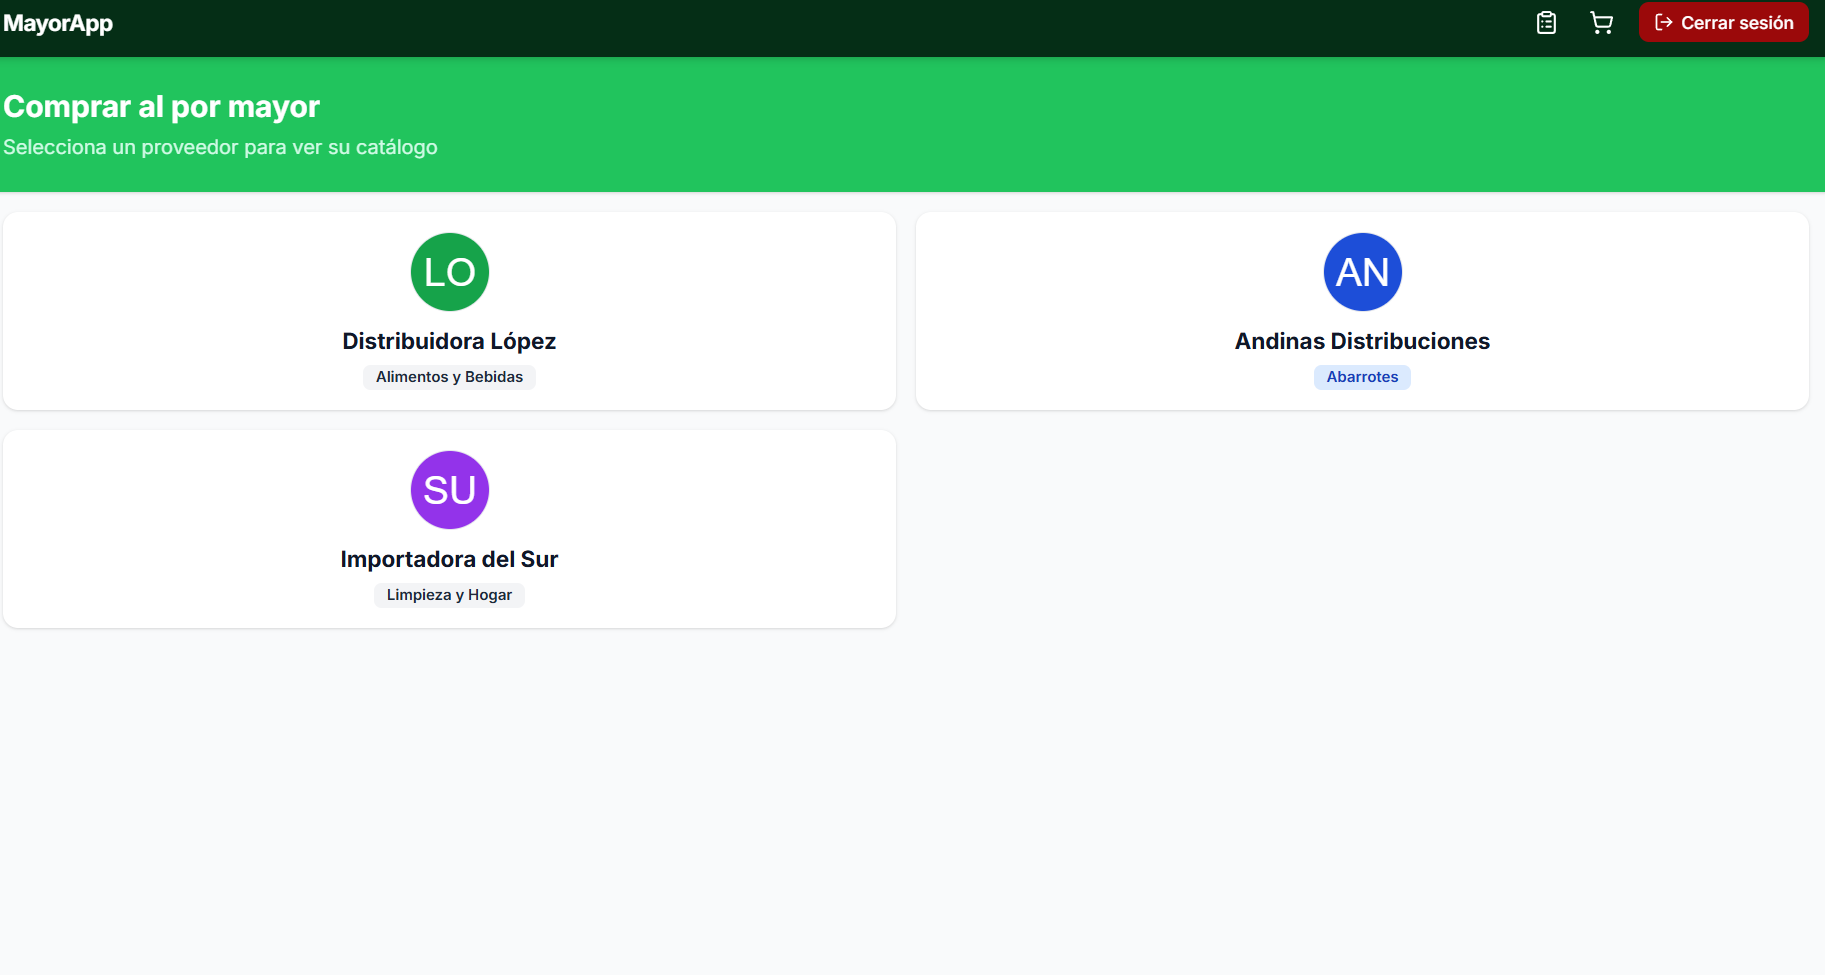
\includegraphics[width=0.9\textwidth]{image17.png}
  \caption*{Tienda -- Marketplace (Comprar al por mayor)}
\end{figure}
\begin{figure}[H]
  \centering
  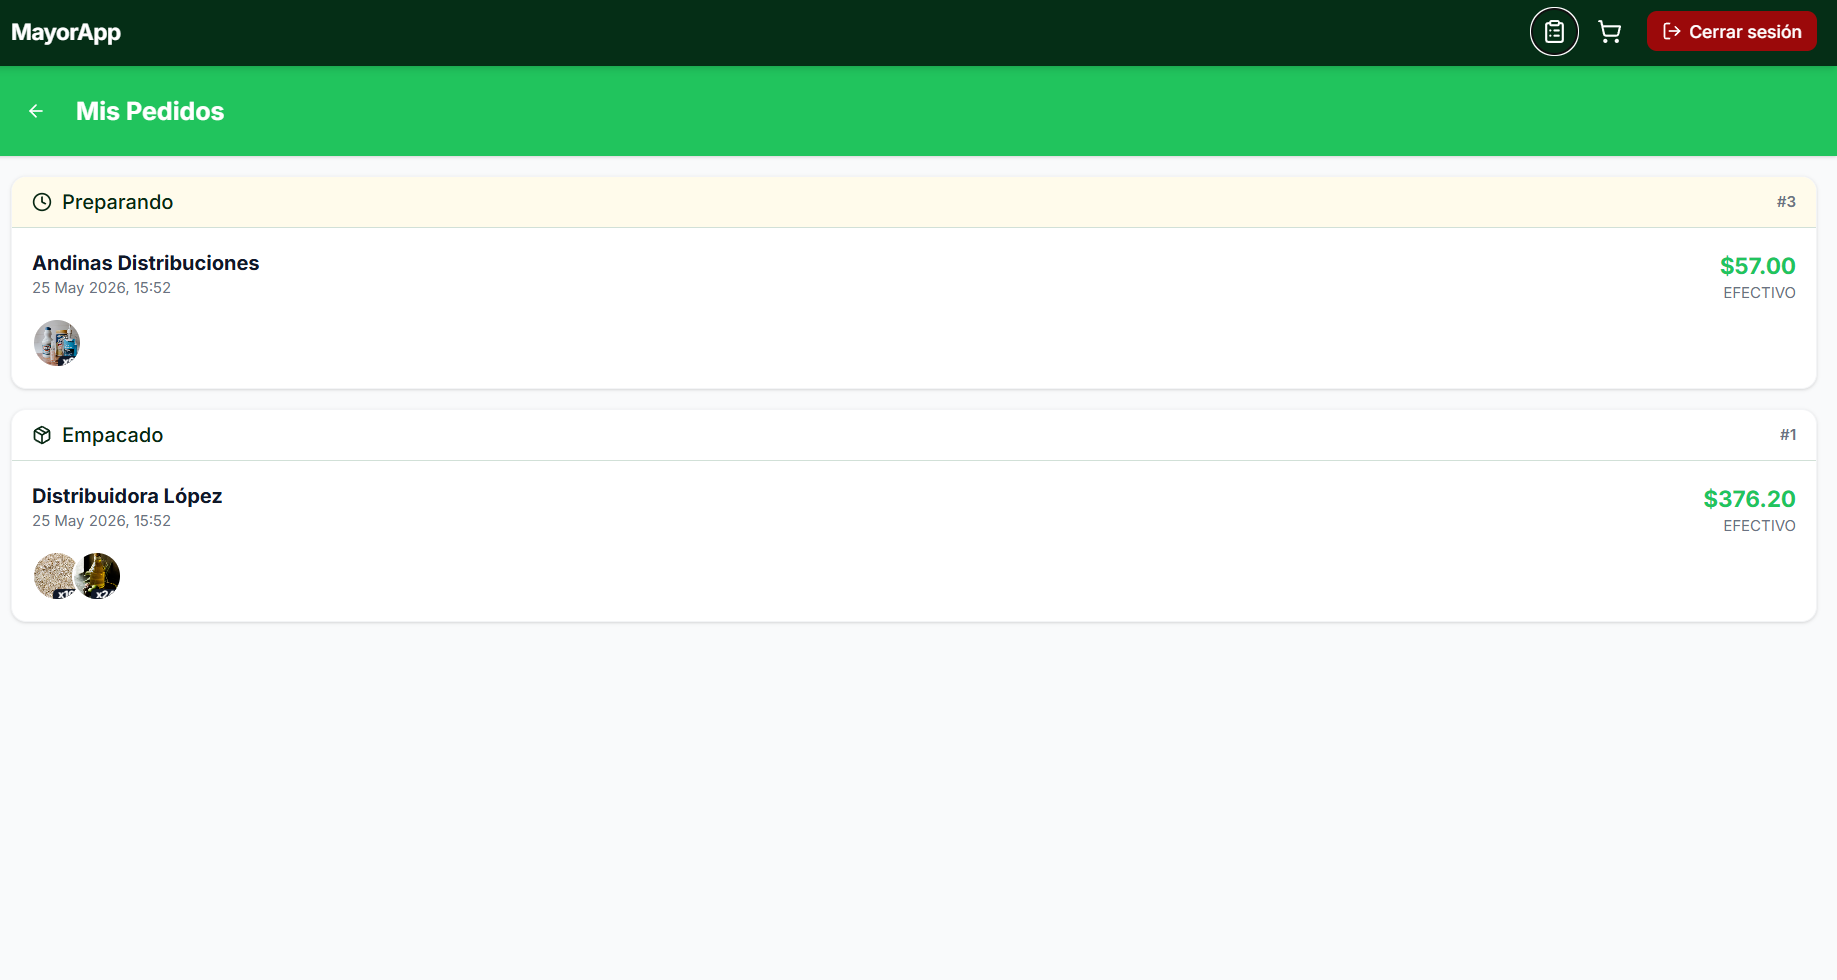
\includegraphics[width=0.9\textwidth]{image18.png}
  \caption*{Tienda -- Mis Pedidos}
\end{figure}
\begin{figure}[H]
  \centering
  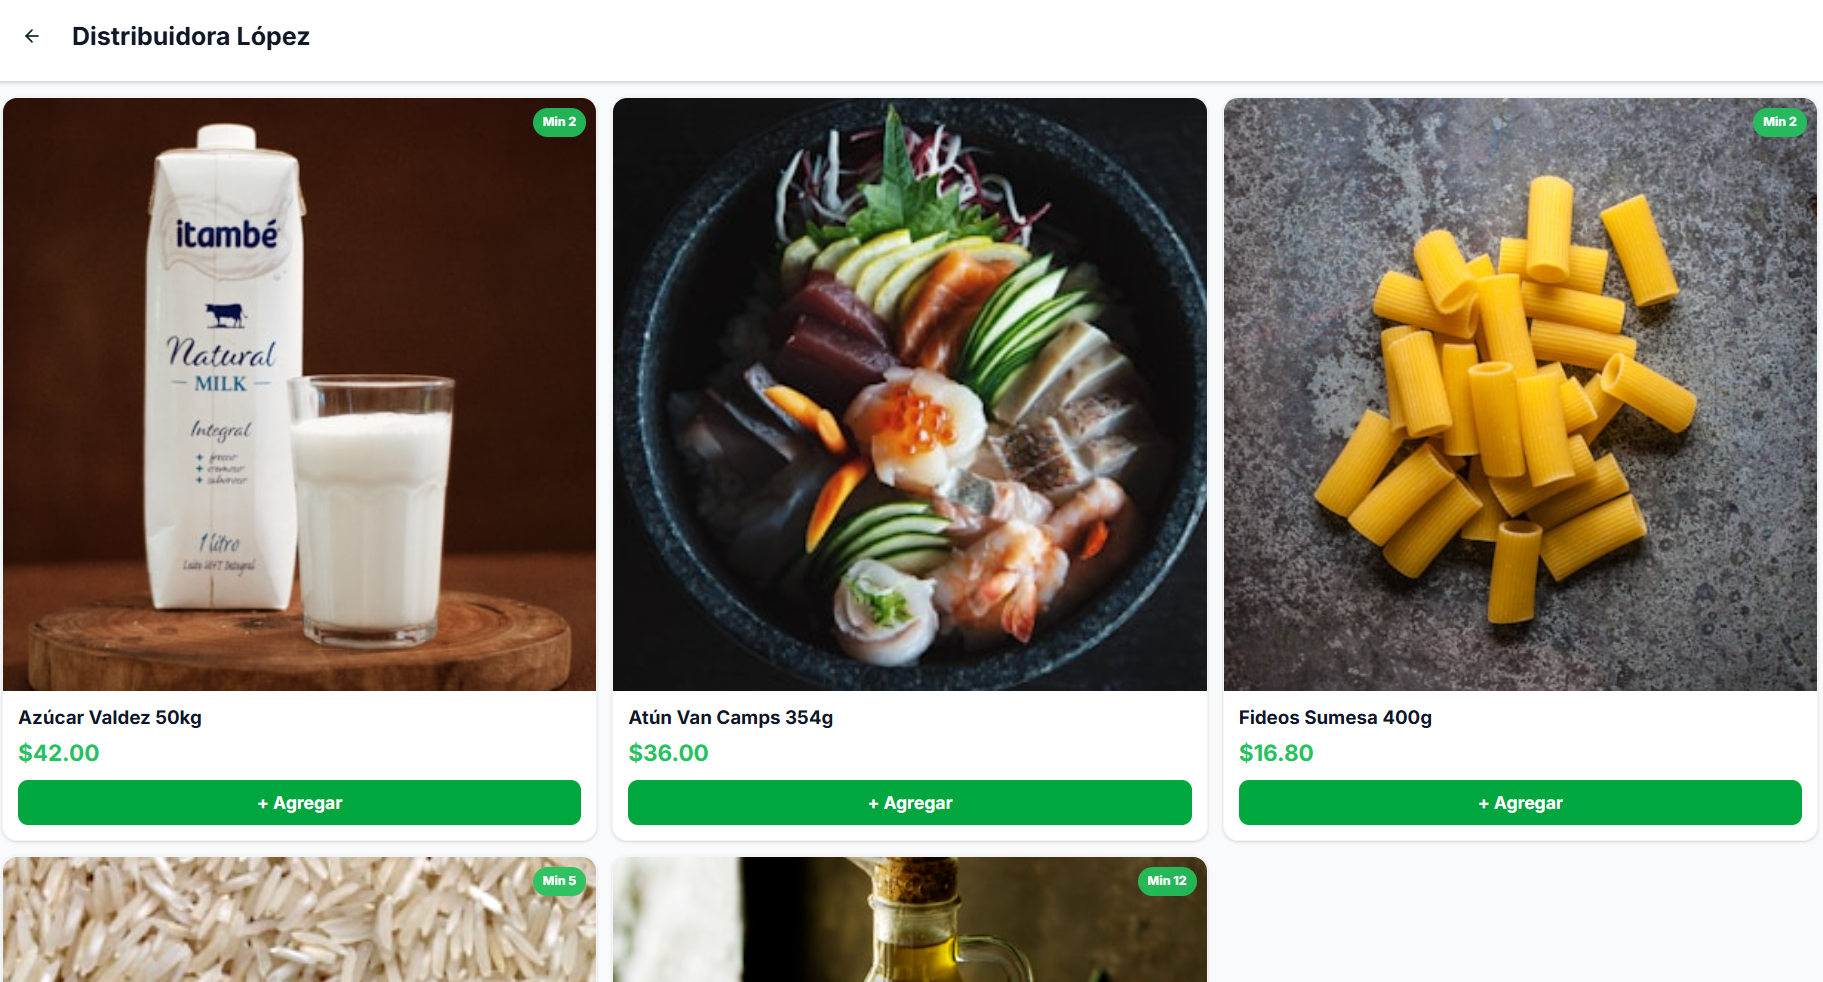
\includegraphics[width=0.9\textwidth]{image19.png}
  \caption*{Tienda -- Catálogo del Mayorista}
\end{figure}
\begin{figure}[H]
  \centering
  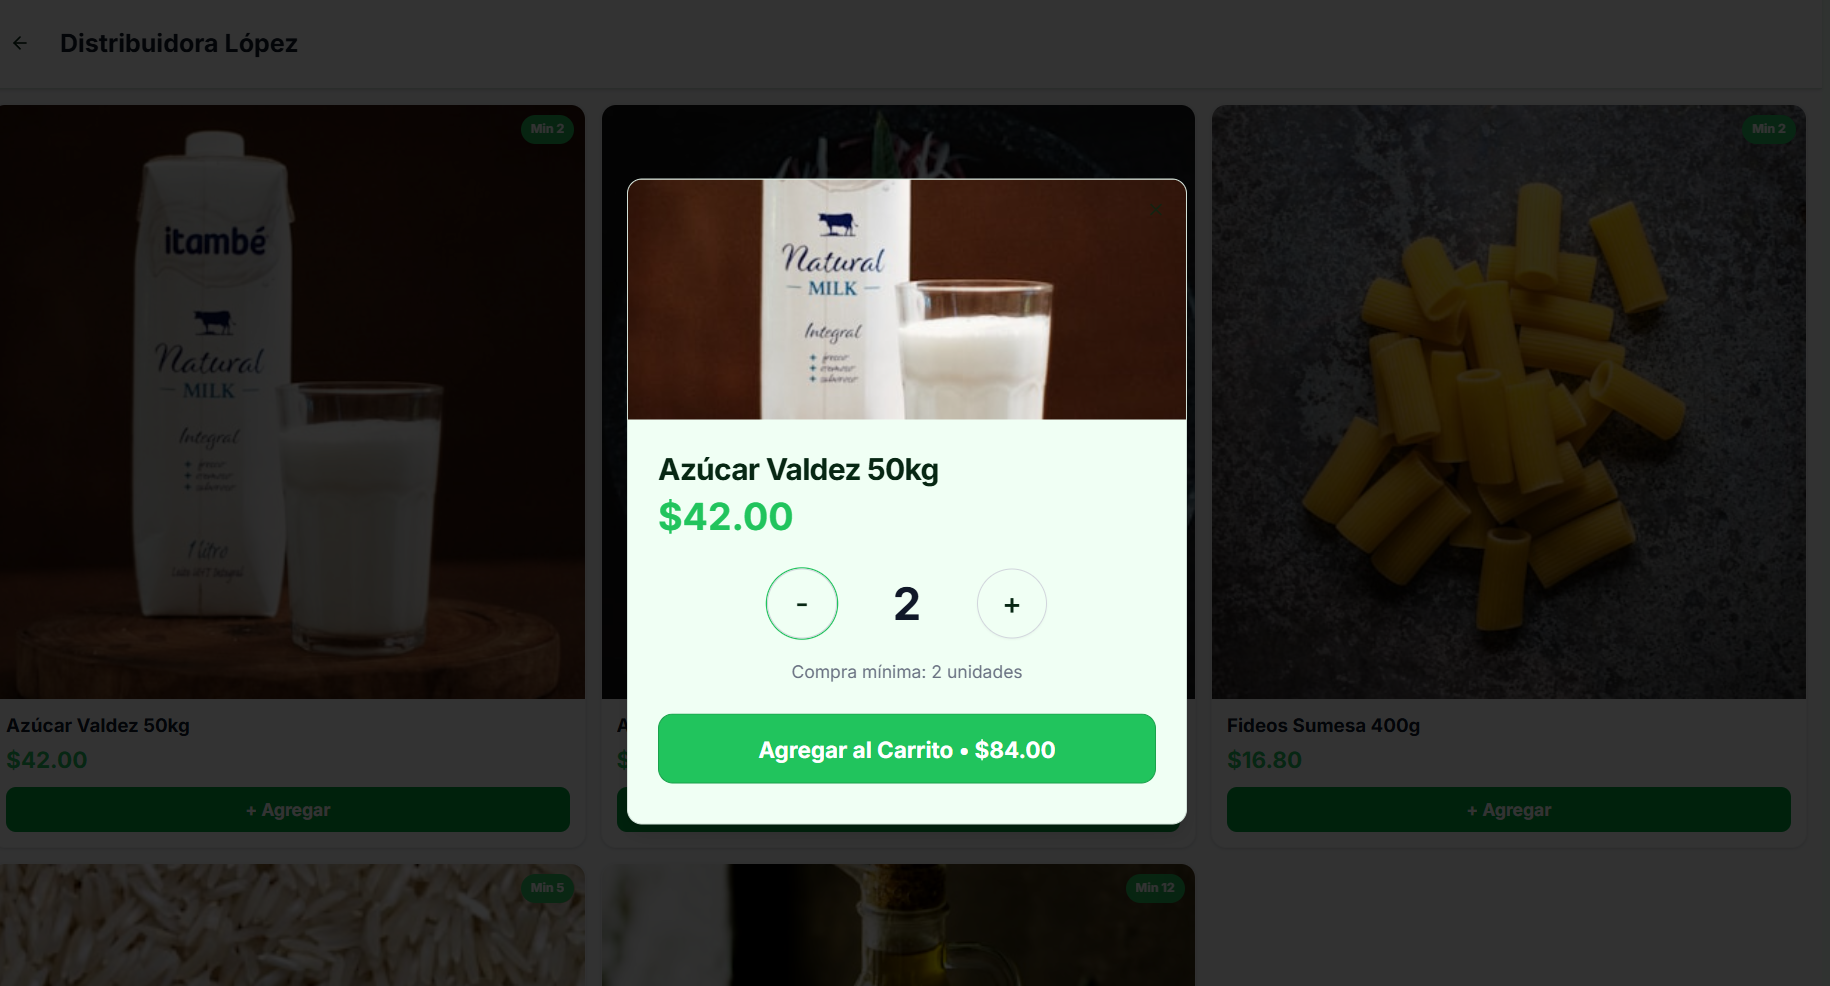
\includegraphics[width=0.9\textwidth]{image20.png}
  \caption*{Tienda -- Selección de Productos}
\end{figure}
\begin{figure}[H]
  \centering
  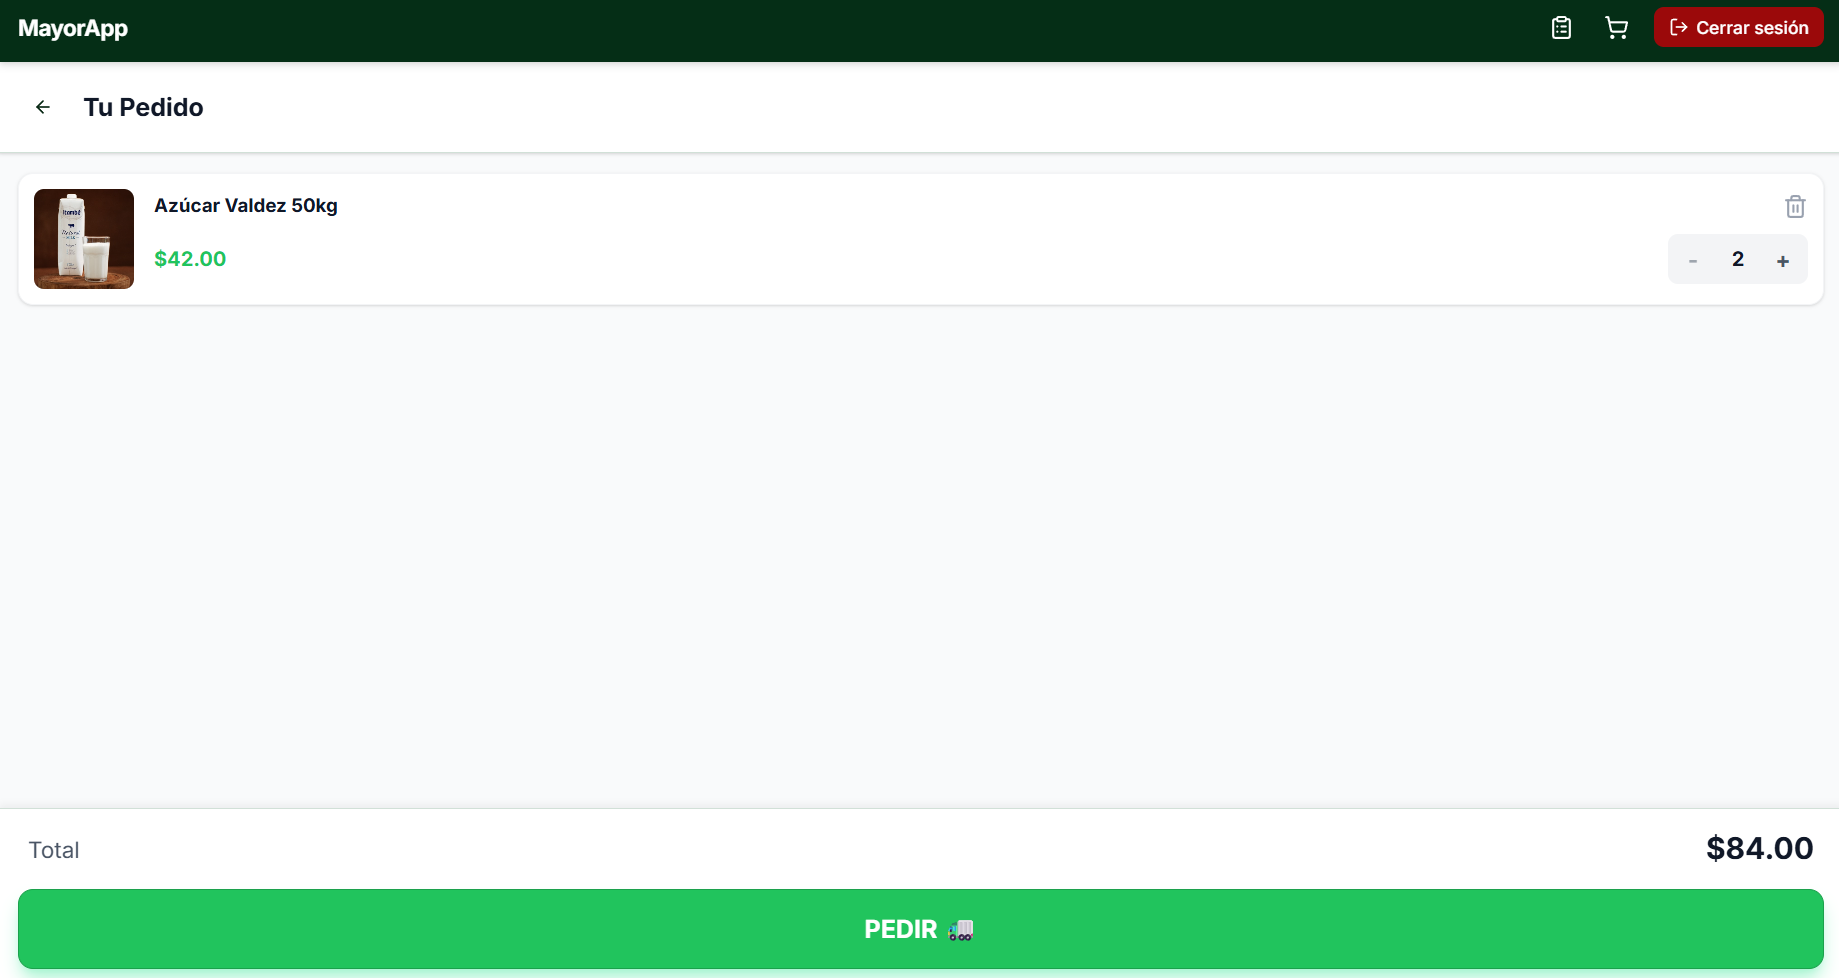
\includegraphics[width=0.9\textwidth]{image21.png}
  \caption*{Tienda -- Tu Pedido (resumen)}
\end{figure}

\paragraph{Vendedor:}

\begin{figure}[H]
  \centering
  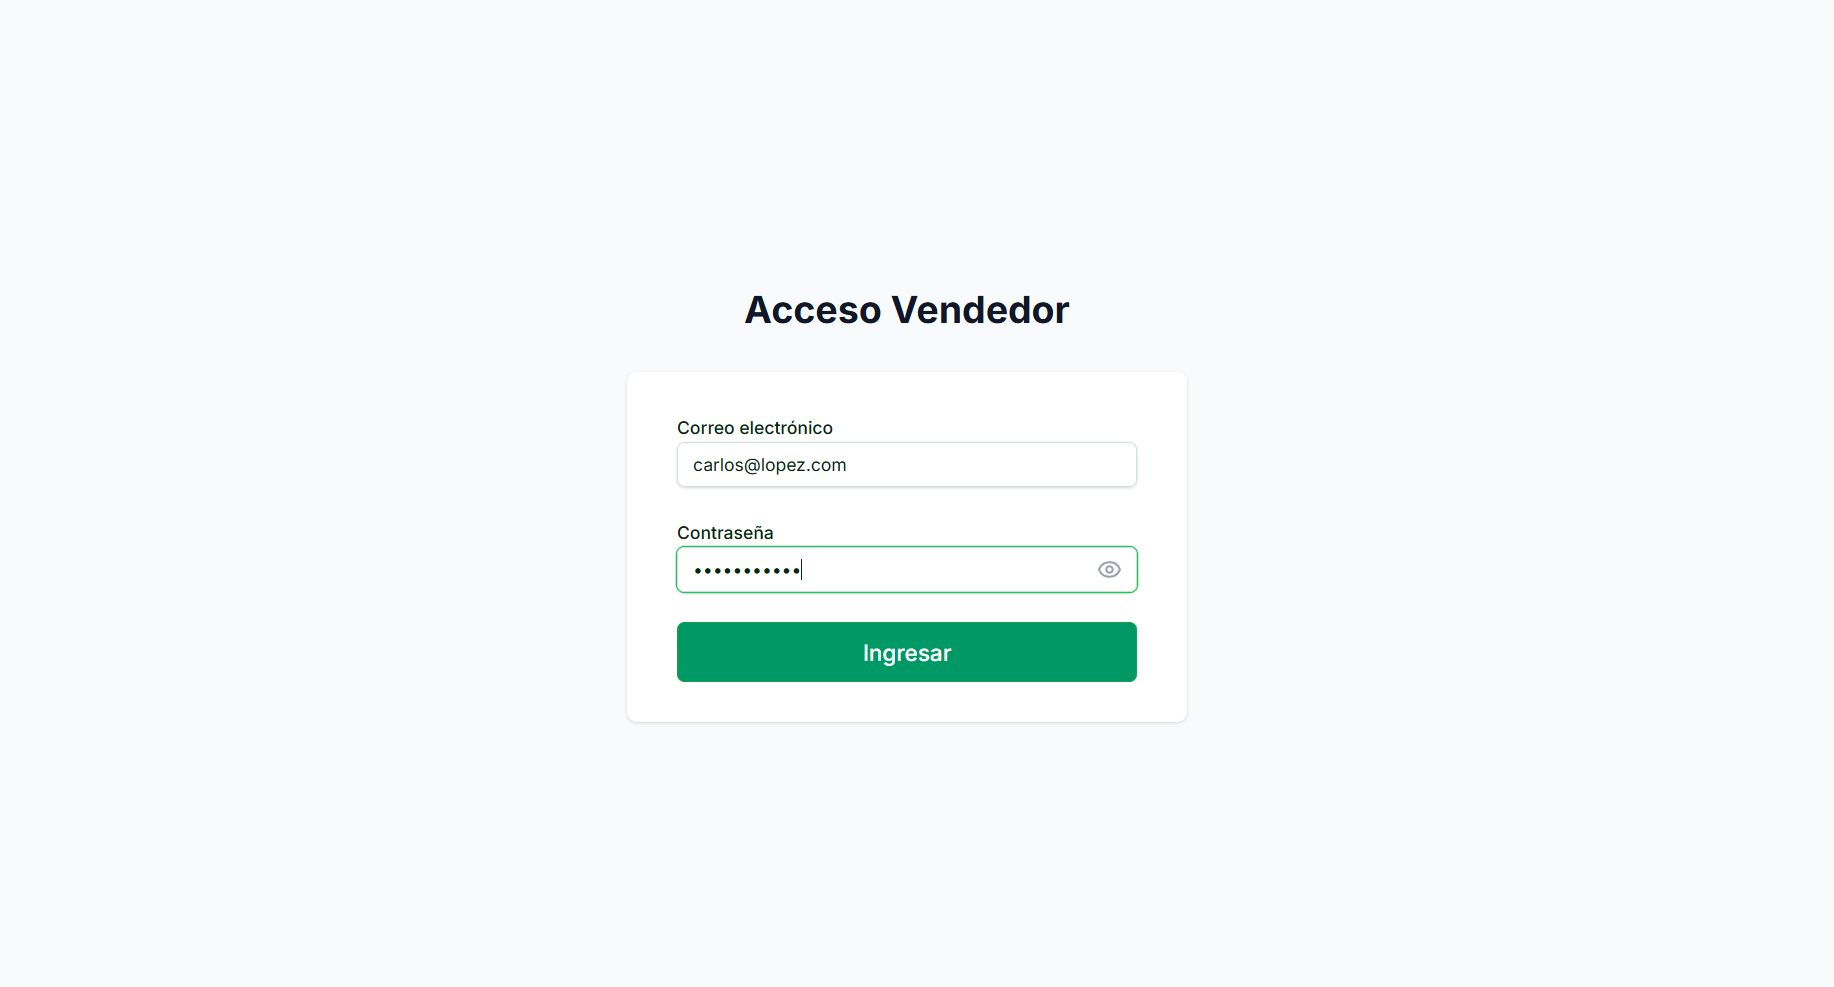
\includegraphics[width=0.9\textwidth]{image22.png}
  \caption*{Vendedor -- Inicio de sesión}
\end{figure}
\begin{figure}[H]
  \centering
  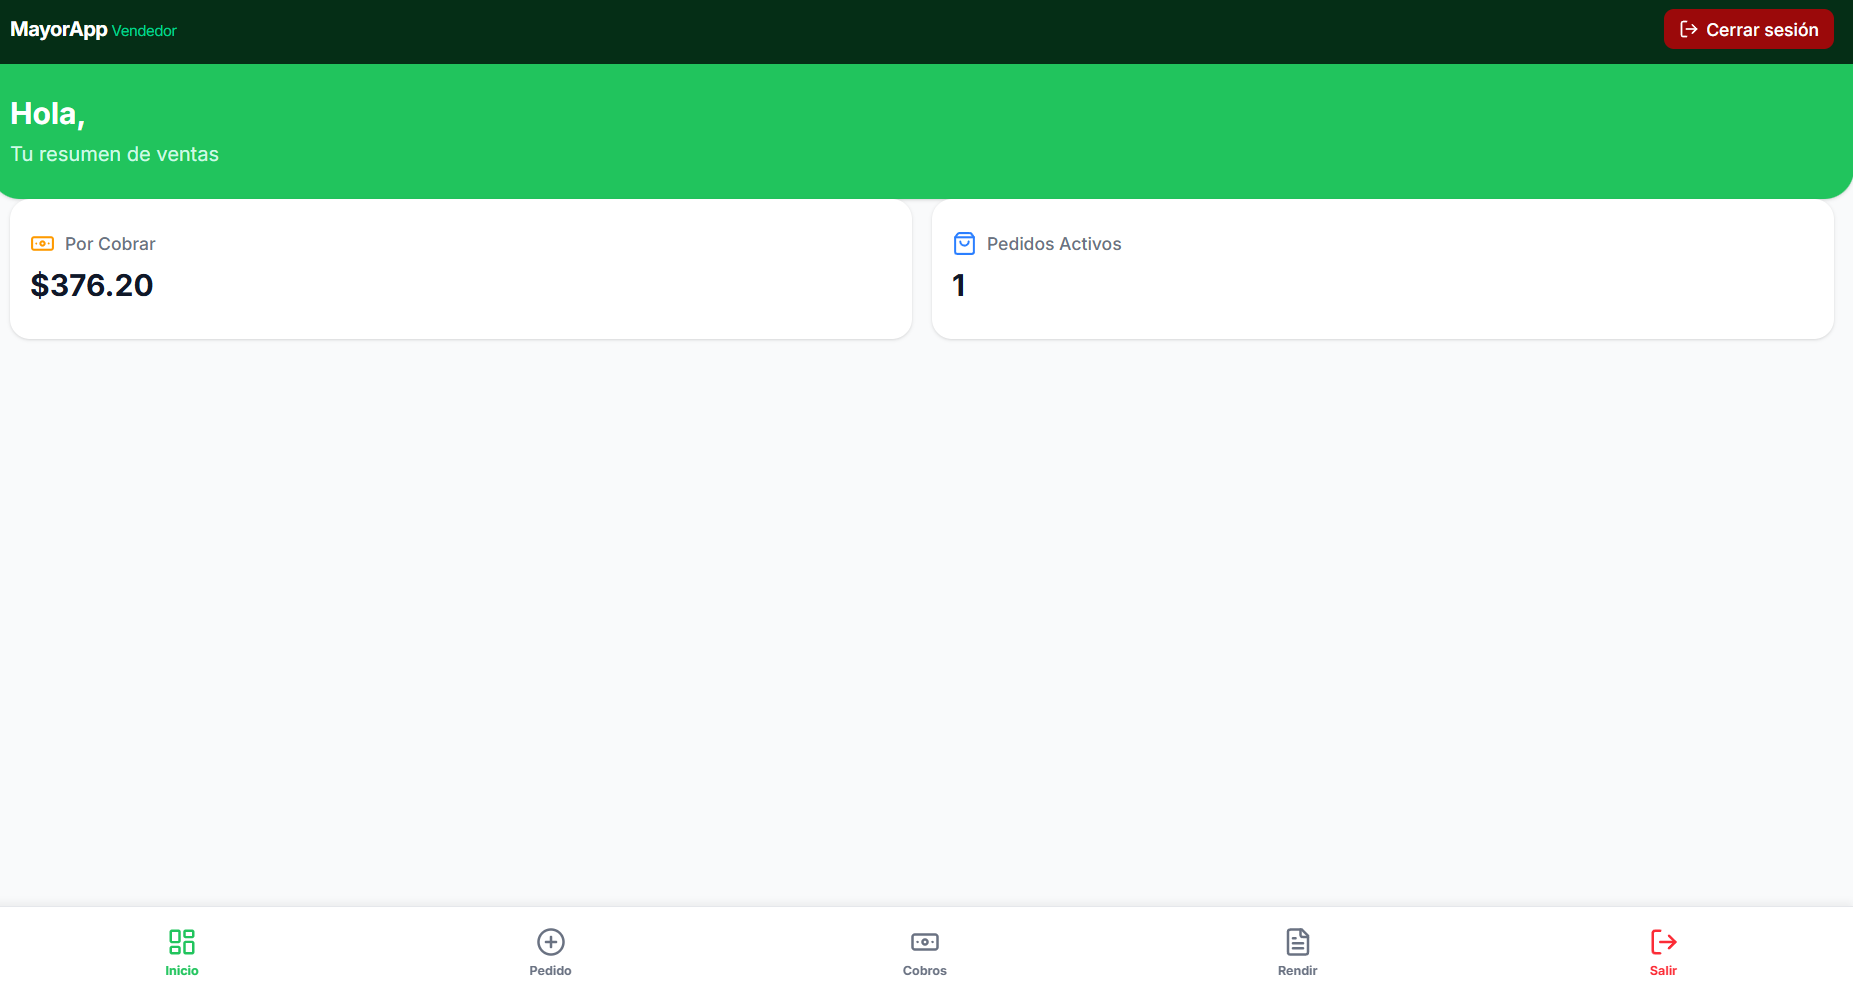
\includegraphics[width=0.9\textwidth]{image23.png}
  \caption*{Vendedor -- Dashboard}
\end{figure}
\begin{figure}[H]
  \centering
  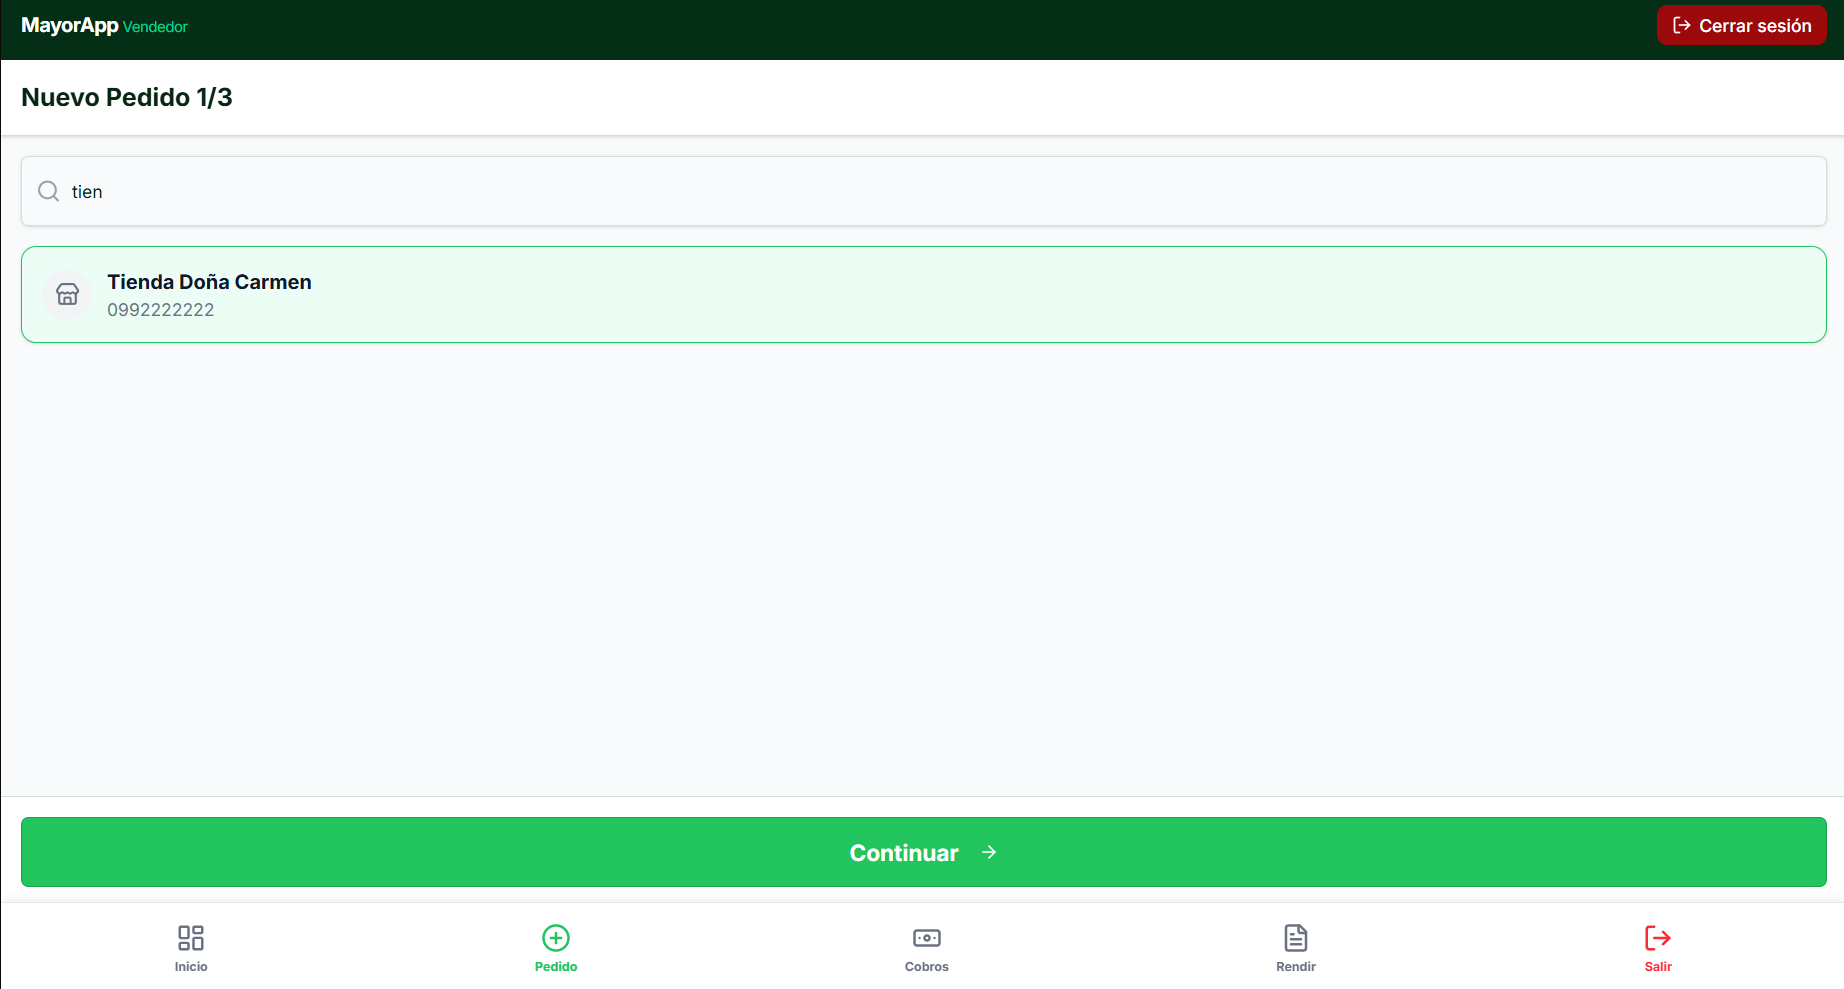
\includegraphics[width=0.9\textwidth]{image24.png}
  \caption*{Vendedor -- Nuevo Pedido (paso 1/3)}
\end{figure}
\begin{figure}[H]
  \centering
  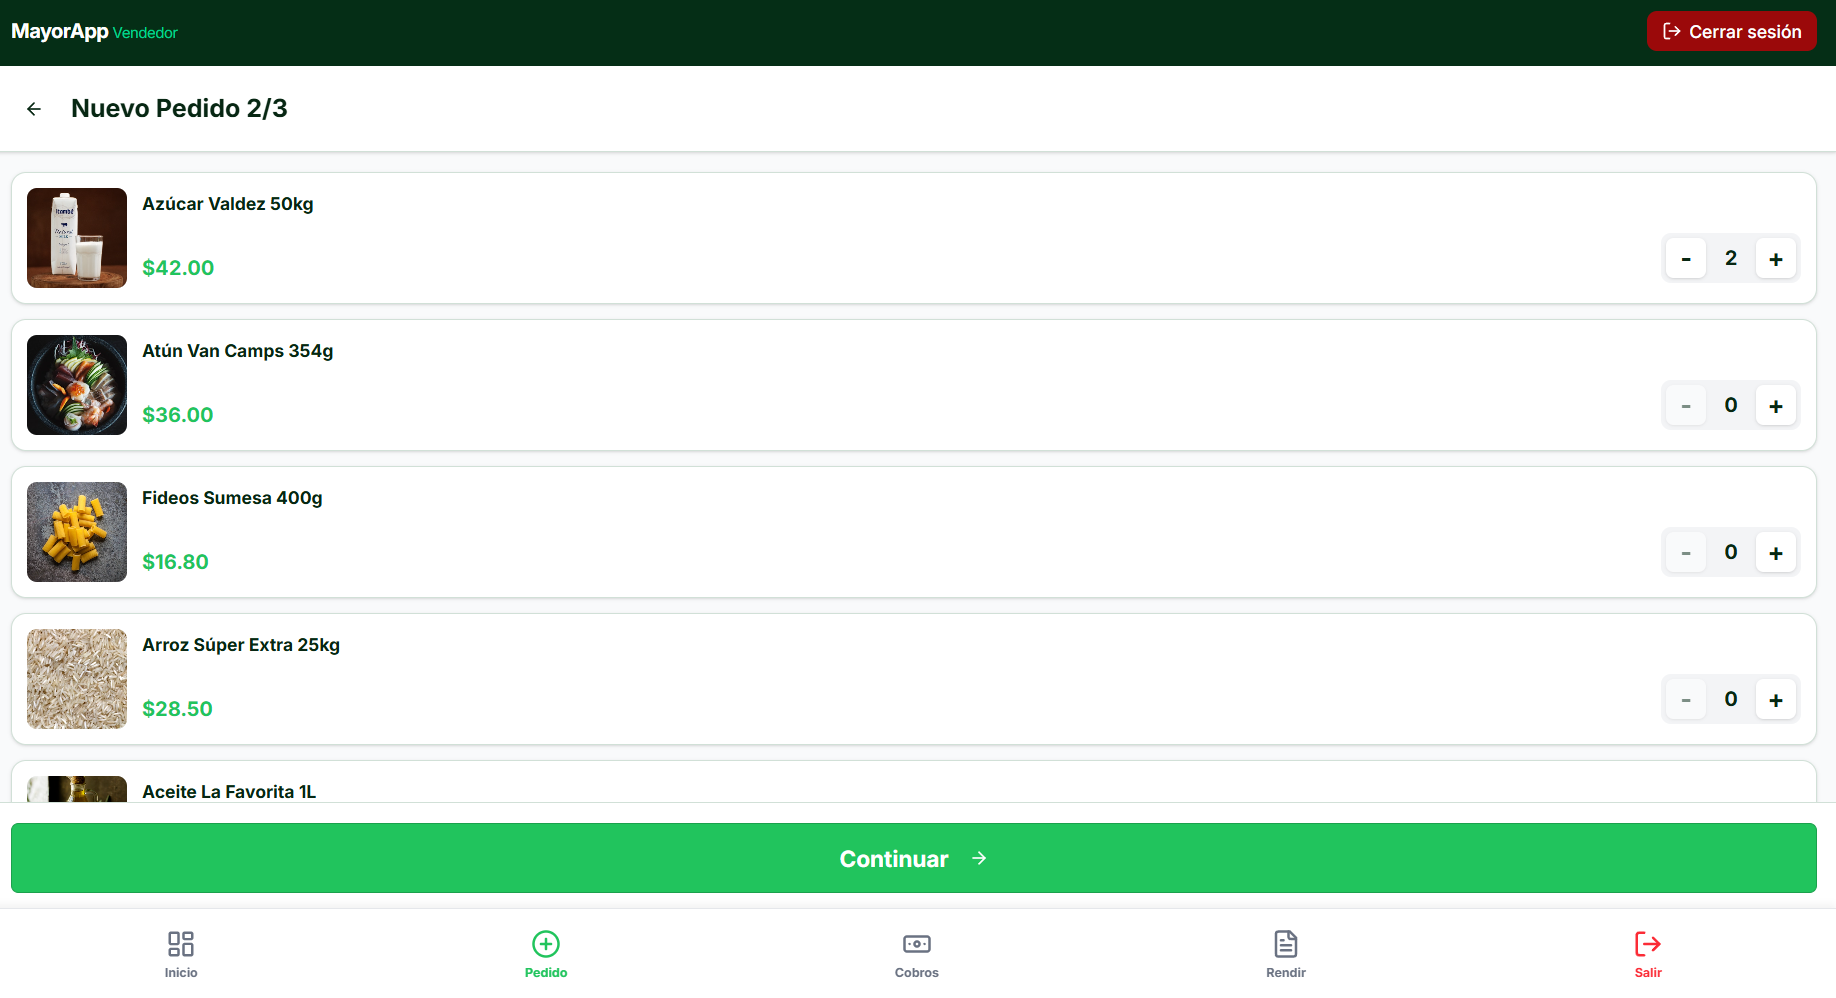
\includegraphics[width=0.9\textwidth]{image25.png}
  \caption*{Vendedor -- Nuevo Pedido (paso 2/3)}
\end{figure}
\begin{figure}[H]
  \centering
  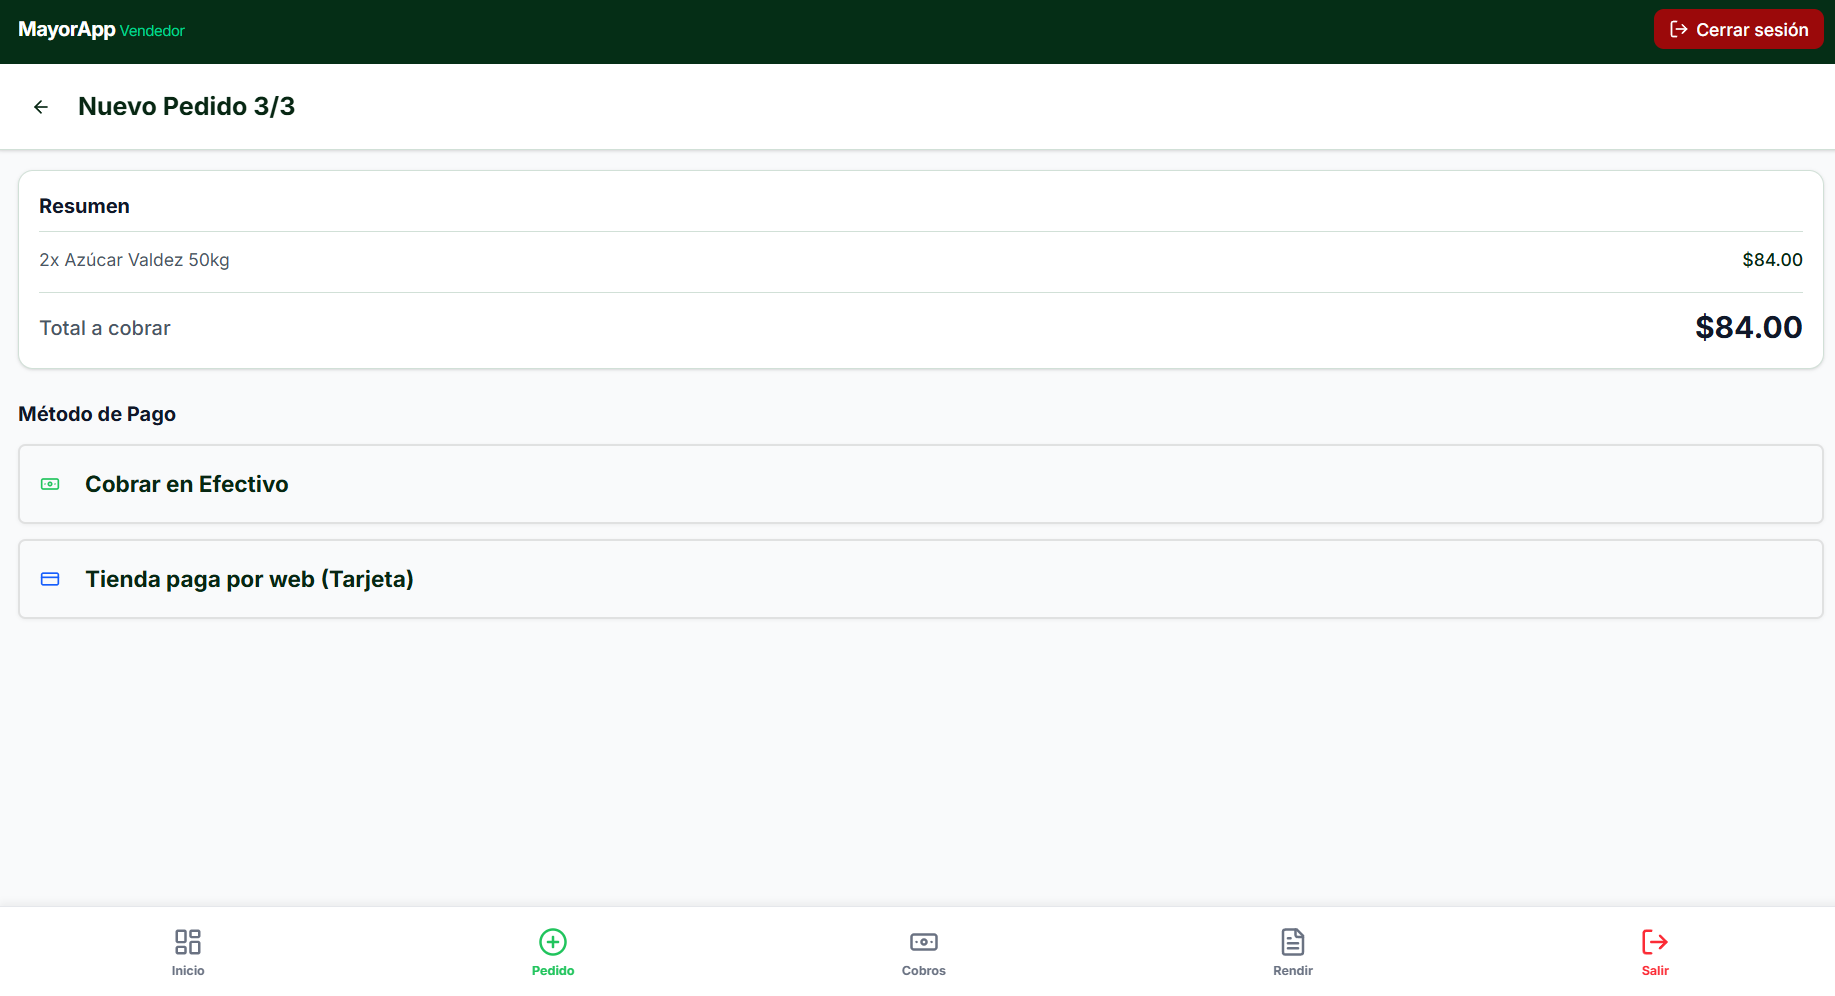
\includegraphics[width=0.9\textwidth]{image26.png}
  \caption*{Vendedor -- Nuevo Pedido (paso 3/3)}
\end{figure}
\begin{figure}[H]
  \centering
  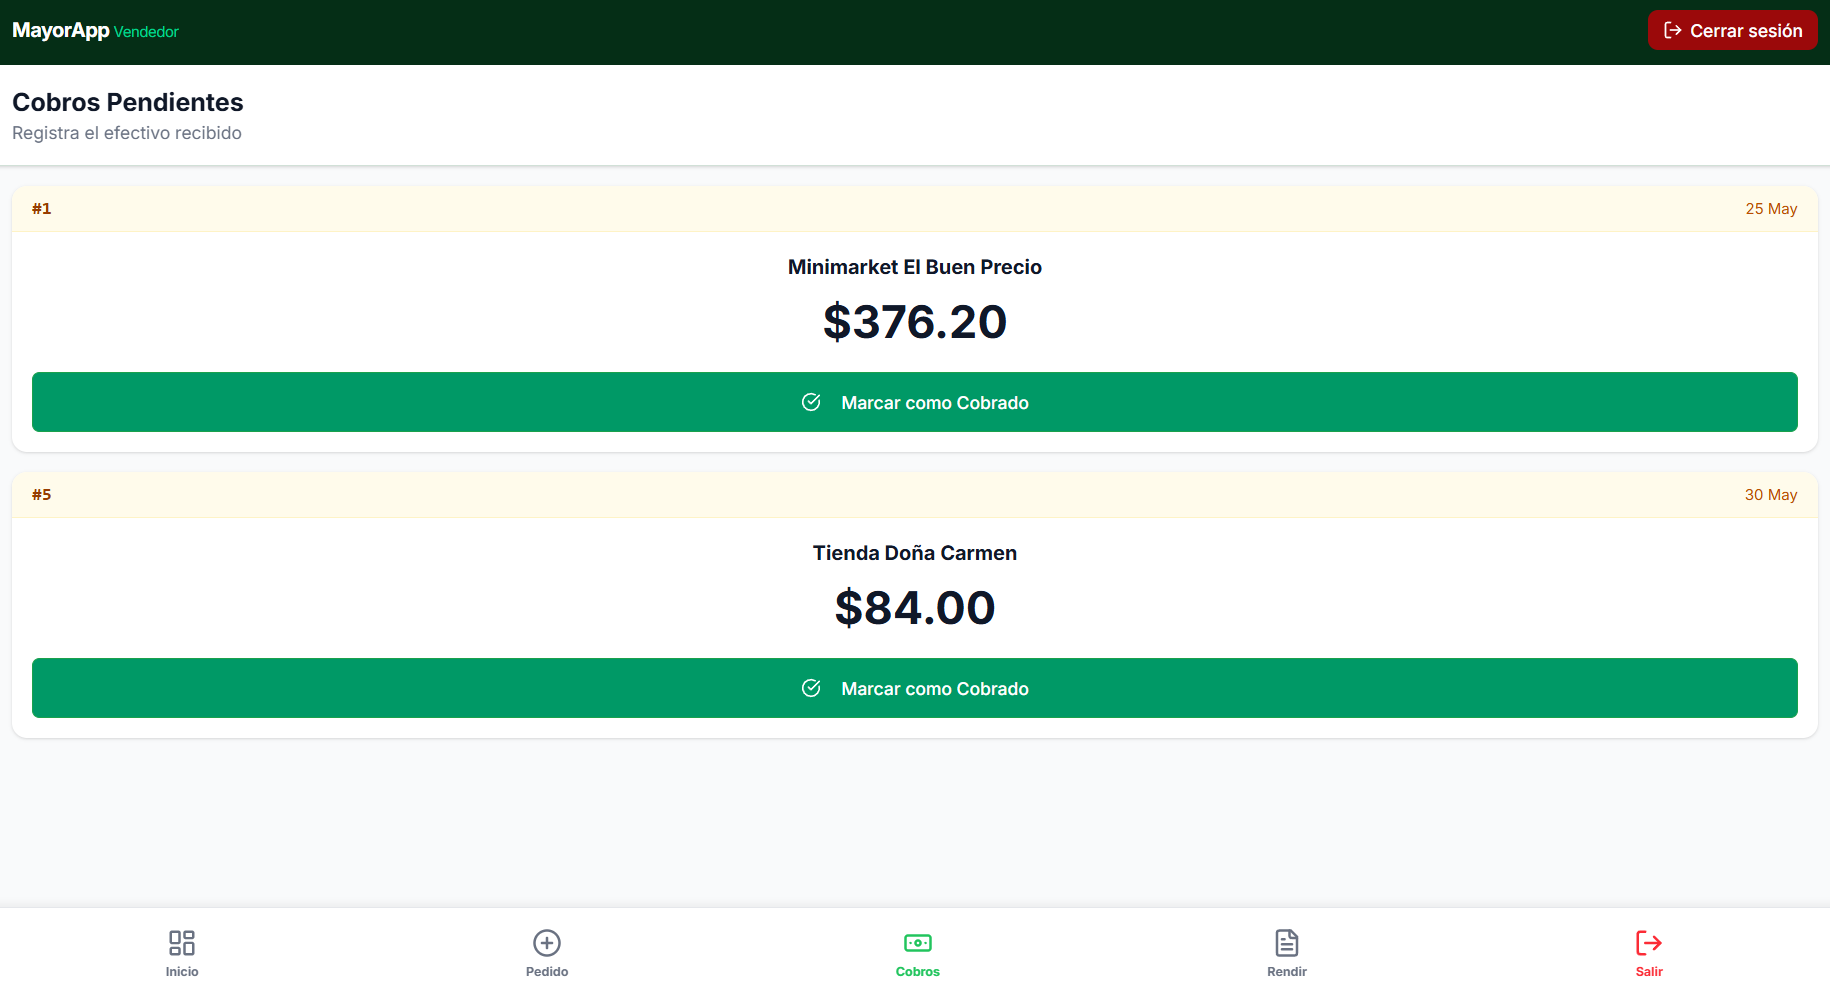
\includegraphics[width=0.9\textwidth]{image27.png}
  \caption*{Vendedor -- Cobros Pendientes}
\end{figure}
\begin{figure}[H]
  \centering
  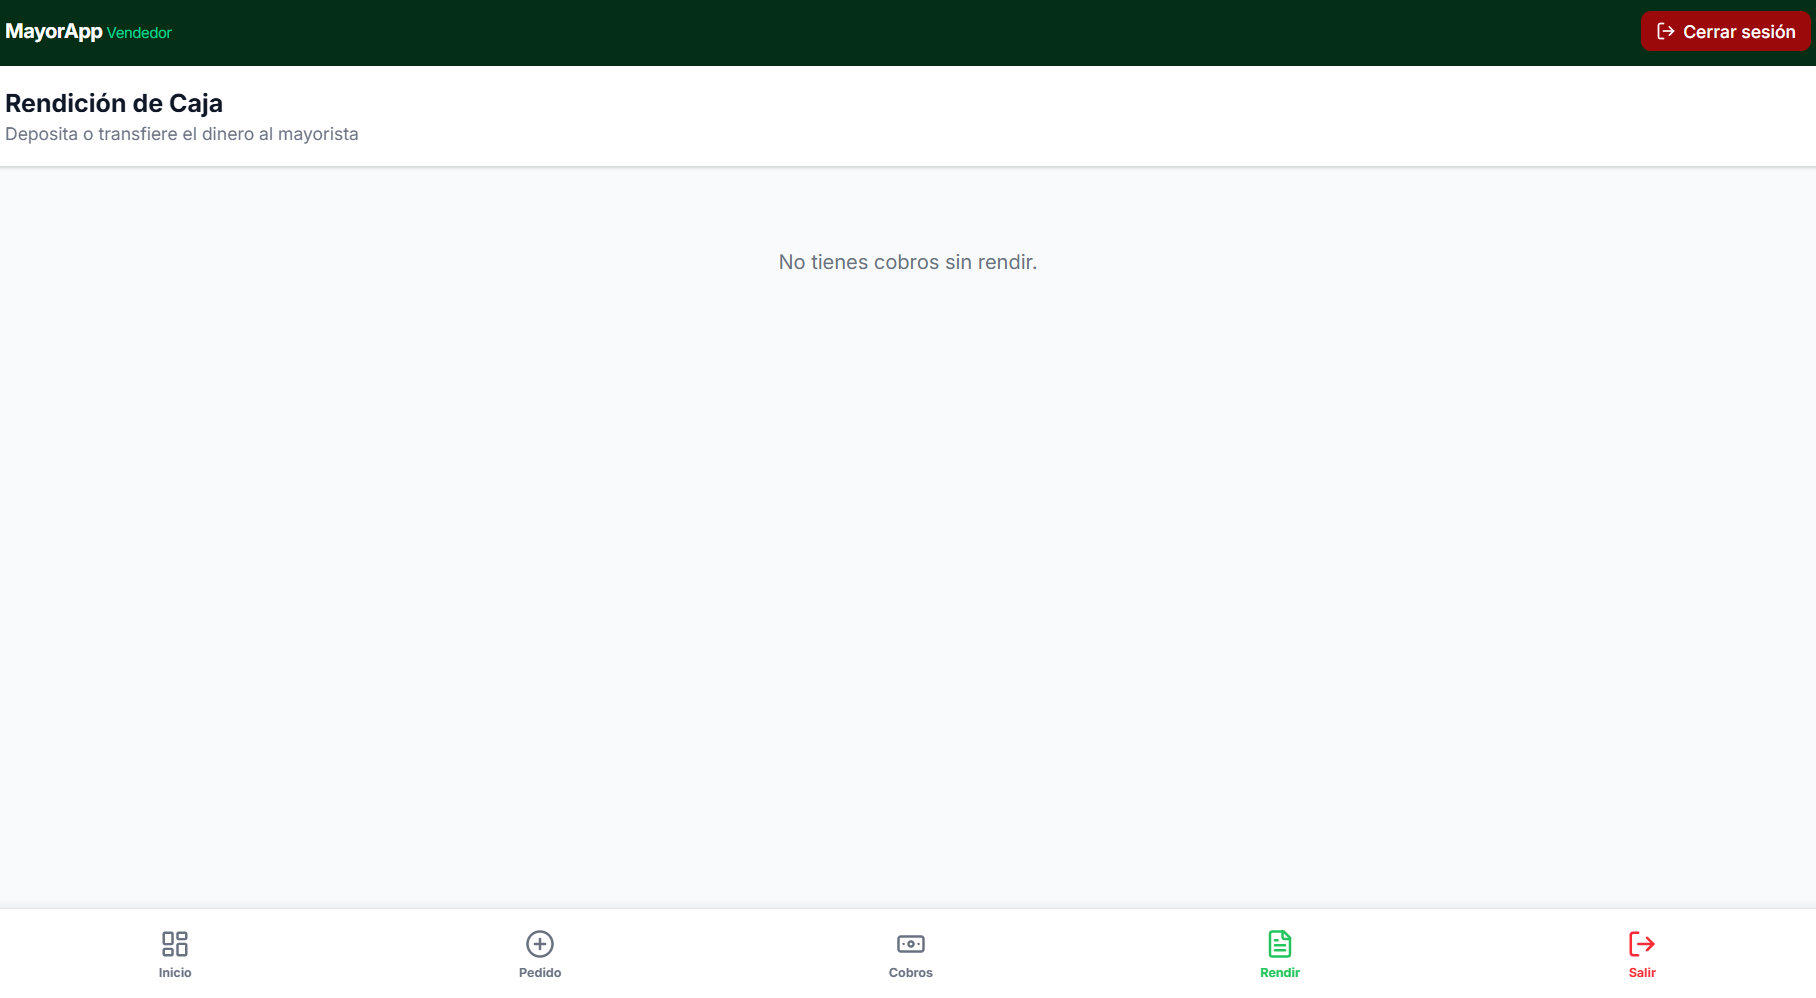
\includegraphics[width=0.9\textwidth]{image28.png}
  \caption*{Vendedor -- Rendición de Caja}
\end{figure}

\paragraph{Administrador:}

\begin{figure}[H]
  \centering
  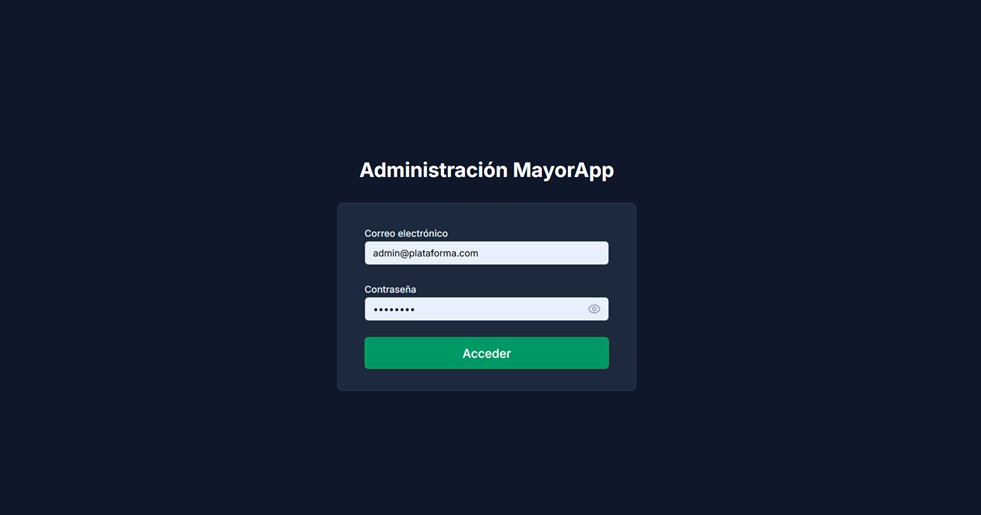
\includegraphics[width=\textwidth, keepaspectratio]{image29.png}
  \caption*{Login -- Administración MayorApp}
\end{figure}

\begin{figure}[H]
  \centering
  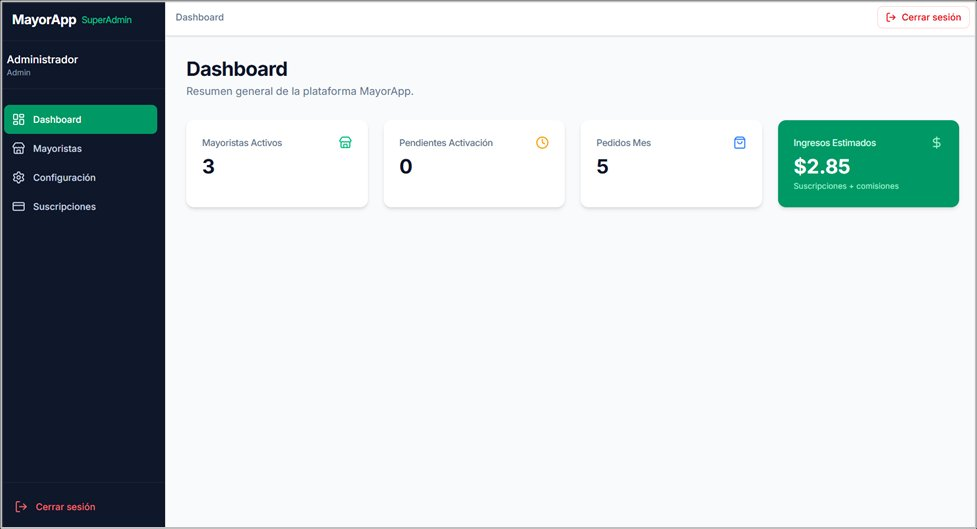
\includegraphics[width=\textwidth, keepaspectratio]{image30.png}
  \caption*{Dashboard}
\end{figure}

\begin{figure}[H]
  \centering
  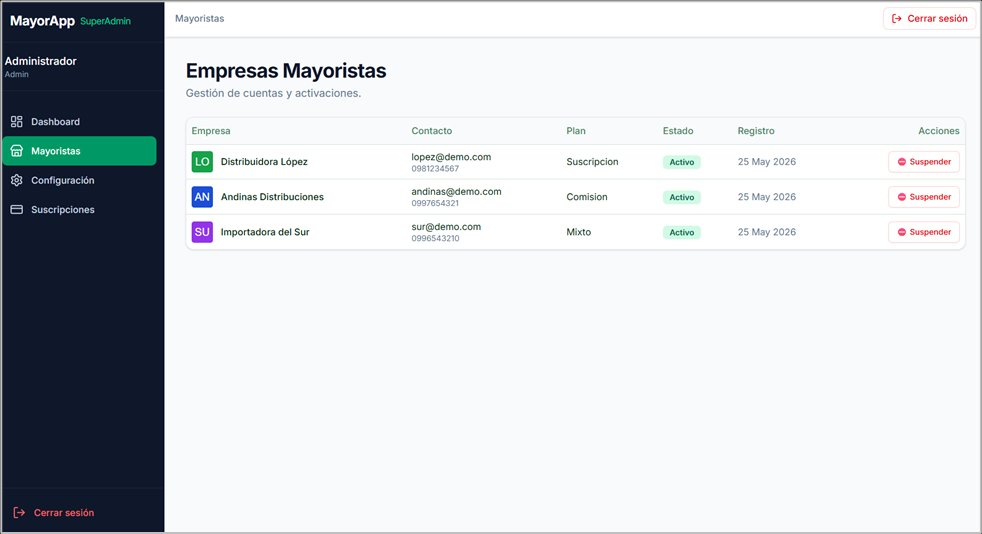
\includegraphics[width=\textwidth, keepaspectratio]{image31.png}
  \caption*{Empresas Mayoristas}
\end{figure}

\begin{figure}[H]
  \centering
  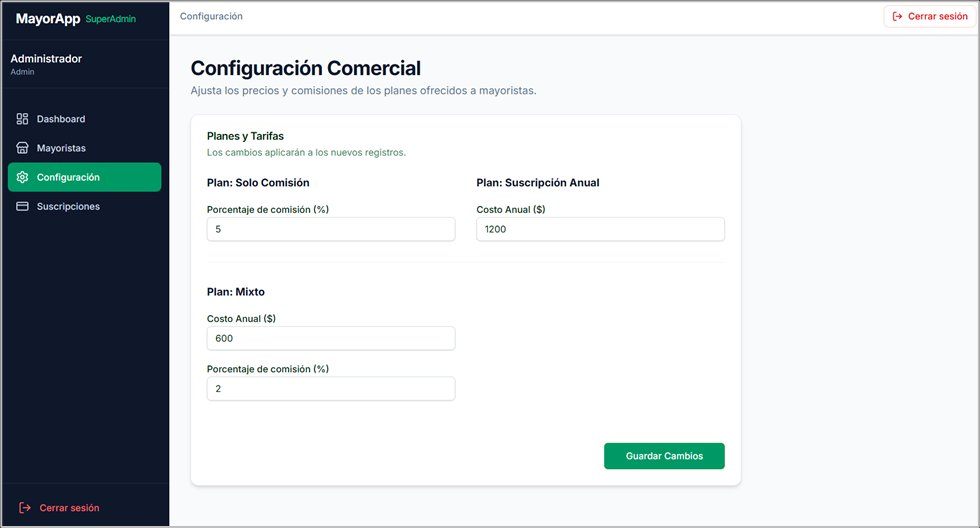
\includegraphics[width=\textwidth, keepaspectratio]{image32.png}
  \caption*{Configuración Comercial}
\end{figure}

\begin{figure}[H]
  \centering
  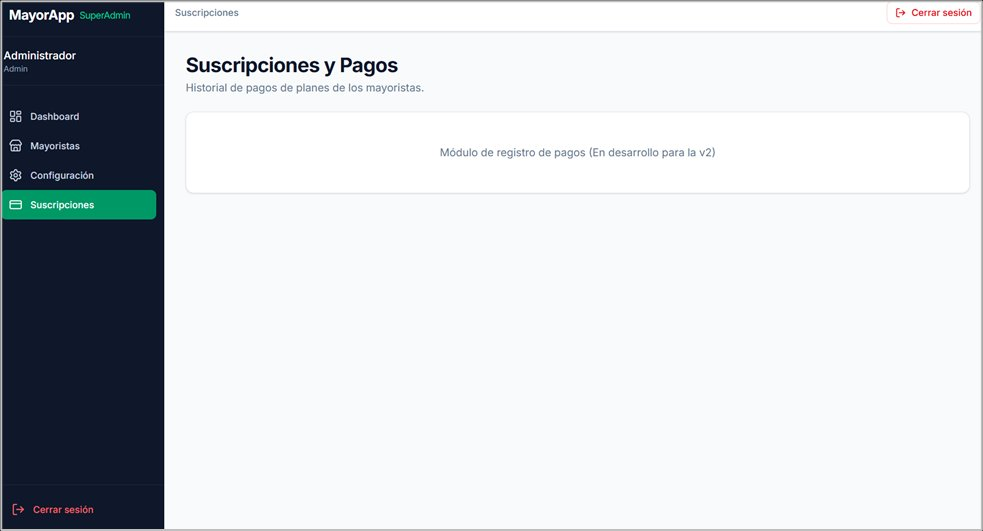
\includegraphics[width=\textwidth, keepaspectratio]{image33.png}
  \caption*{Suscripciones y Pagos}
\end{figure}

\end{document}
